\documentclass[]{article}
\usepackage[spanish]{babel}
\usepackage[utf8]{inputenc}
\usepackage{graphicx}
\usepackage{geometry}
\usepackage{textpos}
\usepackage{fancyhdr}
\usepackage{float}
\usepackage{array}
\usepackage{multirow}
\usepackage{listings}
\usepackage{tikz}
\usetikzlibrary{arrows,shapes,positioning,shadows,trees}


\usepackage[colorlinks=true,linkcolor=black,anchorcolor=black,citecolor=black,filecolor=black,menucolor=black,runcolor=black,urlcolor=black]{hyperref}
\pagestyle{fancy}
\setlength{\headheight}{40pt}
\renewcommand{\headrulewidth}{1pt}
\renewcommand{\footrulewidth}{1pt}

\lhead{\leftmark}
\rhead{\thepage}
\cfoot{}
\lfoot{Plan de Gestión, Análisis, Diseño Y Memoria del Proyecto}

\begin{document}
\begin{titlepage}
	\begin{textblock*}{100mm}(.75\textwidth,-1.5cm)
	Equipo: \textsc{Margaret Hamilton}
    \end{textblock*}
    \begin{textblock*}{100mm}(.66\textwidth,-1.15cm)
    \hspace{-3cm}Contacto:  Julia   716185@unizar.es / Sergio 721057@unizar.es
	\end{textblock*}
    \vfill
	\centering 
\includegraphics[scale=0.3]{figuras/margaret.png}\\[3em]
    \centering \huge \textsc{Proyecto Sota y Rey}\\[1em]
    \centering \large \textsc{Plan de gestión, análisis, diseño y memoria del proyecto}\\[3em]
    \centering \today
\end{titlepage}

\tableofcontents
\newpage


\section{Introducción}

El presente documento recoge el plan de gestión, análisis, diseño y memoria del proyecto de implementación de una aplicación web para jugar partidas de Guiñote online. La aplicación permite jugar a este conocido juego de cartas contra amigos o adversarios desconocidos de su mismo nivel ya sea en uno contra uno o por parejas. Además, si se prefiere, la aplicación ofrece una Inteligencia Artificial a la que poder retar para entrenarse sin necesidad de un contrincante real.\\

La aplicación no se limita a ser una plataforma para jugar partidas de Guiñote, sino que añade componentes de red social y funcionalidades para aumentar el atractivo del juego. El sistema utiliza un registro de perfil de usuario en el que se almacena un historial completo de cada jugador. Además, existirá la posibilidad de visualizar partidas que están siendo jugadas en ese momento en modo espectador. Las funcionalidades que incrementan la jugabilidad de la aplicación se basan en añadir competitividad. Existirá un sistema de ligas al que se pertenece en función de las habilidades del usuario, medidas según el ratio de partidas ganadas y perdidas, y un sistema de torneos de eliminación directa a los que los jugadores podrán inscribirse. Como recompensa al desempeño realizado en los torneos y ligas existirá una divisa virtual que los jugadores ganarán y que podrán utilizar para comprar items en la tienda del juego, que les permitirán personalizar sus partidas.\\

El sistema será accesible desde el navegador (al menos Google Chrome 64). Para que se pueda jugar desde distintos dispositivos la aplicación tendrá una interfaz responsive, adaptándose al tamaño de la pantalla desde la que se juega. Este cambio de dispositivo podrá hacerse incluso durante una partida en curso, siempre que no se agote el tiempo de turno correspondiente. \\

El sistema estará alojado en Amazon AWS como un servidor ejecutado en una instancia virtual de EC2 mientras que todo lo referente al almacenamiento de información (datos jugadores, partidas, elementos de la tienda…) estará almacenado en Amazon Aurora. \\

El desarrollo del proyecto está dividido en dos fases, lo que permite que pueda ser validado y contrastado con el cliente. La primera fase incluirá un prototipo funcional de la aplicación que permitirá jugar partidas individuales, o en modo espectador e incluirá las pantallas de login y perfil de usuario, aunque todavía no tendrá implementada una Inteligencia Artificial funcional y competente. Esta versión del programa será mostrada al cliente el 9 de Abril de 2018.

Como resultado final del proyecto el cliente recibirá la aplicación desplegada en AWS, el código fuente y el resultado de la compilación para la plataforma objetivo. Además, el cliente recibirá un manual técnico completo y una memoria resumen del proceso de desarrollo. La fecha de entrega del producto terminado es el 1 de Junio de 2018.\\

\clearpage

\subsection{Estructura del documento}
En la sección \ref{organiz} se describe la organización del equipo de trabajo, incluyendo un organigrama de la empresa. A continuación, en la sección \ref{planes} se detalla el plan de gestión del proyecto. Esta sección incluye una primera parte relativa a cómo se llevarán a cabo las distintas tareas a lo largo del proyecto (subsección \ref{procesos}) y una segunda referente a los planes (subsección \ref{pl}), en la que se detallan el plan de gestión de configuraciones, el de despliegue, aseguramiento de la calidad y el plan de trabajo especificado en un diagrama de Gantt. Se incluye en la sección \ref{analisis} una descripción detallada de los requisitos funcionales y no funcionales del sistema, así como el diseño del sistema, detallado mediante una serie de diagramas. Finalmente, en la sección \ref{memoria} se describe en detalle el desarrollo del proyecto.

\section{Organización del proyecto}
\label{organiz}

Para incentivar el trabajo en paralelo en proyecto, se han creado diferentes grupos de trabajo identificados por las tareas que conllevan:

\begin{figure}[h]
	\centering 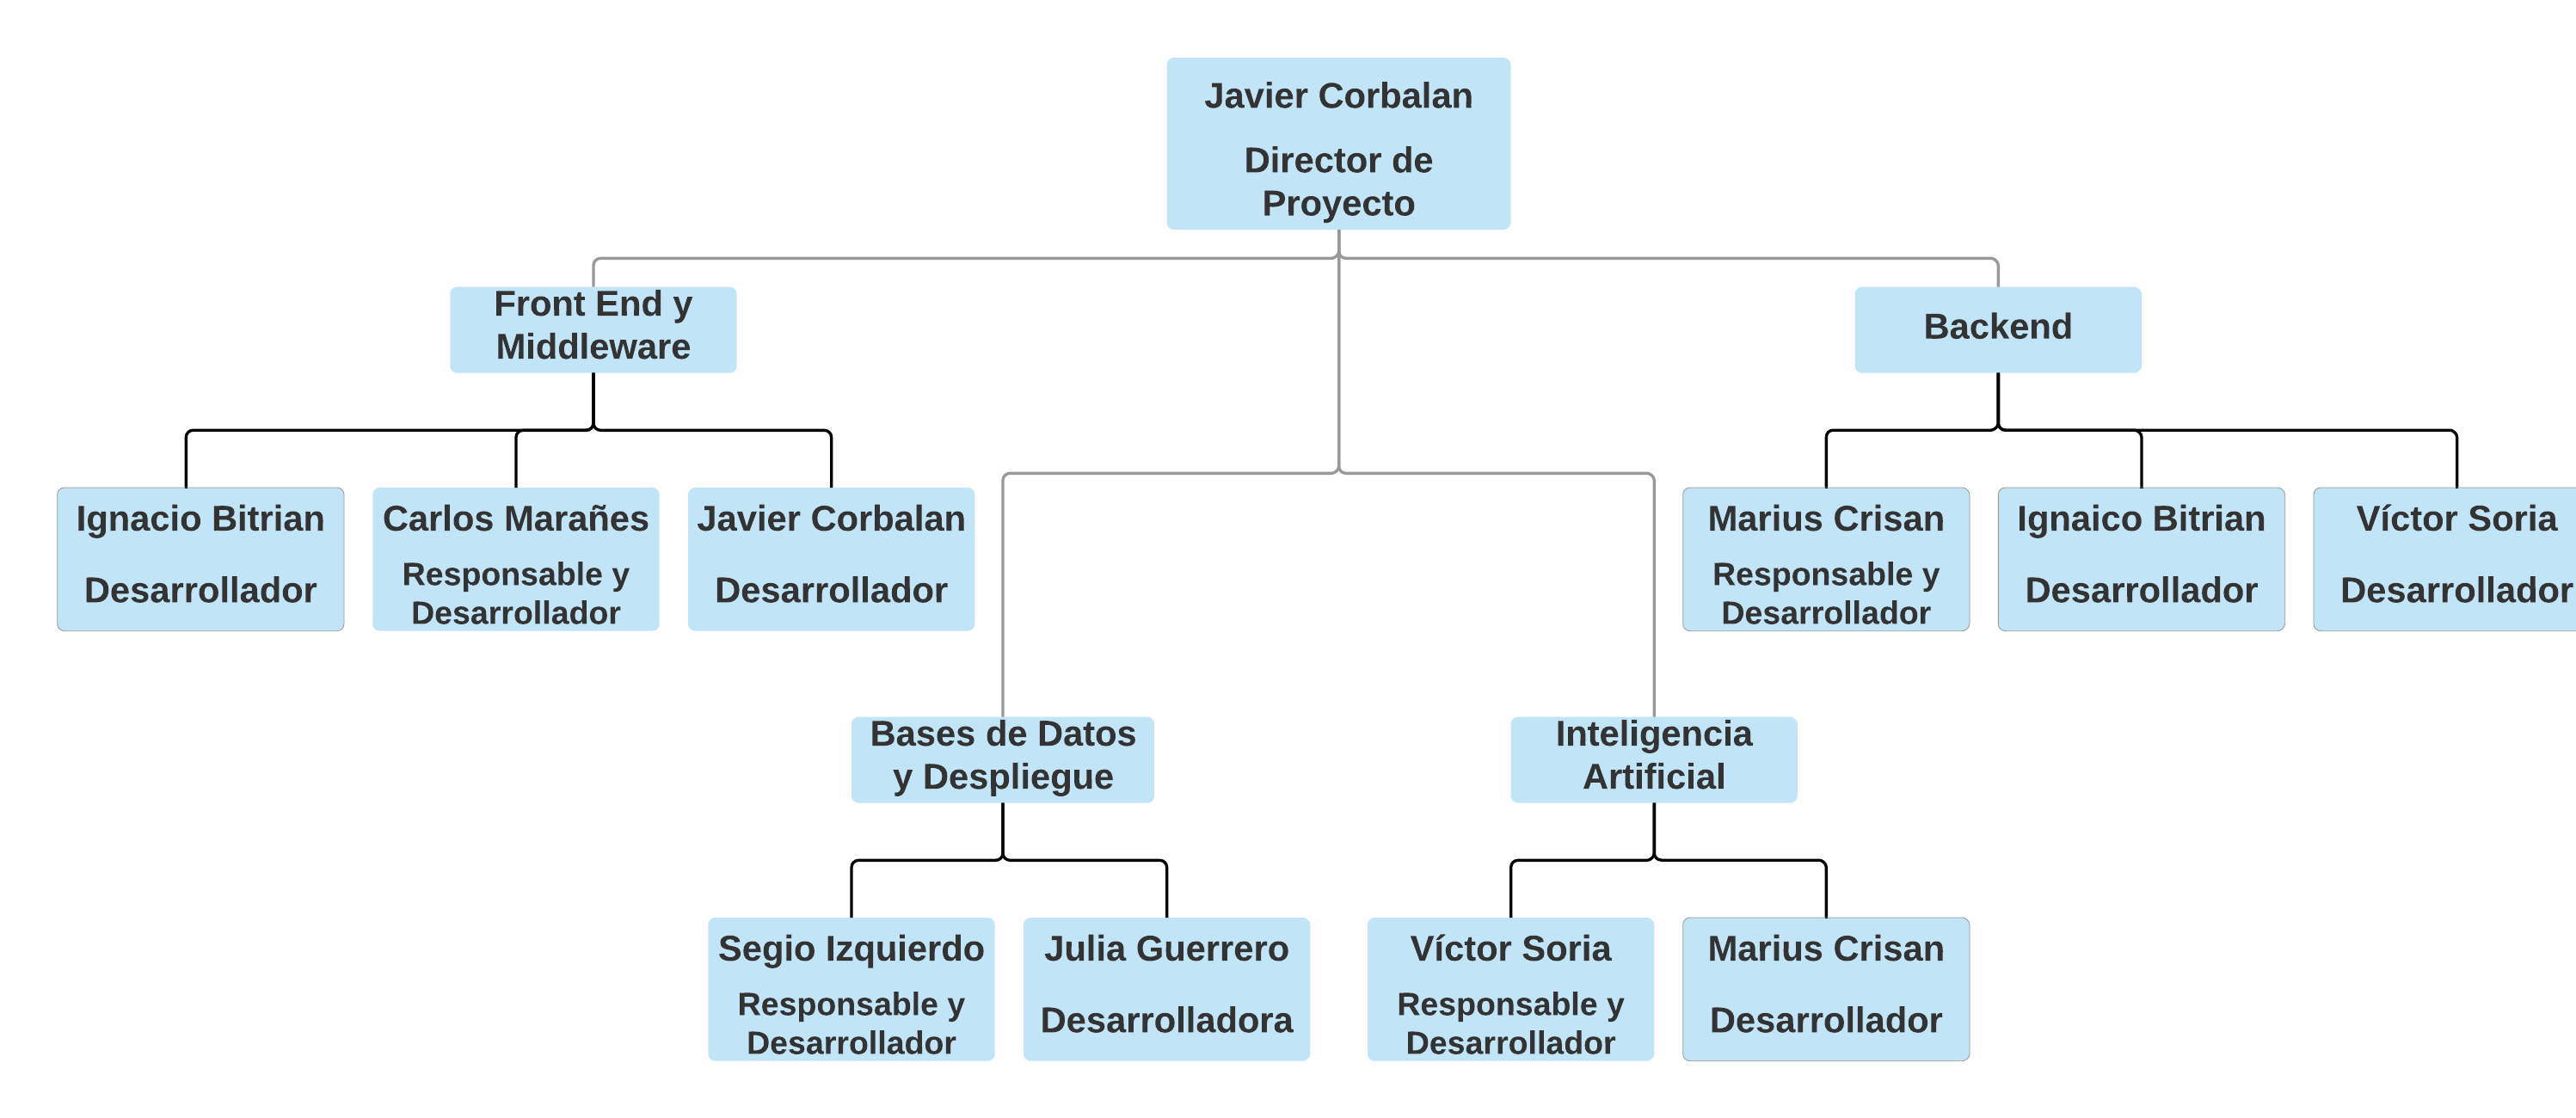
\includegraphics[scale=0.6]{figuras/organigrama.png}
\end{figure}


\begin{enumerate}
\item Desarrollo del Frontend y Middleware: Incluye el desarrollo de la interfaz y las vistas de la aplicación, además de la gestión de la comunicación entre los jugadores y servidor durante el desarrollo la partida.
	
\newpage
\item Despliegue e implementación de la base de datos: Incluye el análisis y diseño de la base de datos, gestión de los datos de carácter personal de los usuarios acorde con la LOPD\footnote{\href{http://www.agpd.es/portalwebAGPD/canaldocumentacion/informes_juridicos/reglamento_lopd/index-ides-idphp.php}{Ley Orgánica de Protección de Datos}} , despliegue de la aplicación y mantenimiento.

\item Desarrollo de la inteligencia artificial: Incluye el análisis del juego, diseño e implementación de un agente de inteligencia artificial.

\item Desarrollo del Backend: Implementación de los servicios web, tratamiento de peticiones, generación de páginas dinámicas y la lógica del juego.

\end{enumerate}

El rol de director del proyecto corre a cargo de Javier Corbalán. La elección del director se ha llevado a cabo a través de una votación de mayoría simple.

\section{Plan de gestión del proyecto}
\label{planes}
\subsection{Procesos}
\label{procesos}

El proyecto está dividido en dos iteraciones, cada una de ellas posee cinco fases: requisitos, análisis, diseño, implementacion y pruebas. En la primara iteración se va a desarrollar el funcionamiento de una partida tanto individual como por parejas y la página web con las pantallas de login y perfil de usuario. En la segunda iteración se va a desarrollar el resto de funcionalidades del sistema, que incluyen la inteligencia artificial, torneos, tienda, entre otros.  Cada fase de cada iteración tiene una duración máxima de una semana, excepto la fase de recogida de requisitos que tiene una duración inferior y que solo se lleva a acabo al inicio del proyecto.
A lo largo del proyecto el equipo se divide en los grupos de desarrollo: bases de datos y despliegue, backend, frontend y middelware e IA. En cada uno de ellos la participación es flexible pero se mantiene de forma fija a un responsable.

\subsubsection{Procesos de inicio del proyecto}
\label{inicio}

Al iniciar el proyecto, cada grupo de desarrollo adquiere las herramientas necesarias para el desarrollo del proyecto. Las principales herramientas son el entorno de desarrollo IntelliJ, creando una cuenta gratis de estudiante y una cuenta de GitHub para poder llevar a cabo el control de versiones del código y documentación del proyecto. Además, se adquiere un certificado TLS gratuito obtenido através del servicio "Let's Encrypt". \\

Además, el equipo  de bases de datos y despliegue debe registrarse en Amazon AWS con la cuenta de estudiante para la contratación de un servicio cloud en Amazon AWS y realizar un estudio para finalmente adquirir un dominio web.  Al finalizar el proyecto estos recursos son traspasados al cliente. \\

Si aparece algún otro recurso necesario cuya adquisición necesite una aportación económica debe ser notificado al director y aprobado por este antes de contratar dicho recurso.\\

Dado que el proyecto integra un gran número de tecnologías y capas que conforman la arquitectura web, es necesario realizar un estudio de viabilidad de las tecnologías escogidas antes de realizar la adquisición del software de desarrollo, este estudio requiere  5 horas de trabajo entre todos los grupos.  En un principio el desarrollo del proyecto se realiza sobre JavaEE, JSP, WebSockets, JavaScript, Bootstrap y MySQL. Como una parte del equipo de desarrollo posee cierta experiencia en el desarrollo web, no tanto en la utilización de estas herramientas, es necesario que se lleve a cabo un proceso de aprendizaje inicial. Este proceso requiere un número mínimo de horas para permitir al equipo comenzar con el desarrollo del proyecto. No obstante, a lo largo del proyecto la formación y la adquisición de experiencia son fundamentales.\\

En aquellas tecnologías donde el equipo de desarrollo no posee ninguna experiencia, como WebSockets, JavaScript , JSP,  entre otros, se requiere un esfuerzo extra por parte del equipo para auto-formarse mediante la lectura de libros, tutoriales y la documentación pertinente.\\

\begin{itemize}
	\item Tanto Carlos Marañés como Javier Corbalán se tienen que formar en Javascript, Websockets y Phaser.io a través del uso de ejemplos y documentación en línea.
	\item Julia Guerrero y Sergio Izquierdo deben formarse en HTML/CSS y JSP con documentación en línea y  con la ayuda de los miembros del equipo que tienen experiencia en esa tecnología.
    \item El equipo entero se va a formar en la dinámica de trabajo con AWS gracias a la experiencia de Sergio Izquierdo y tutoriales en línea.
\end{itemize}

\subsubsection{Procesos de ejecución y control del proyecto}

Una de las funciones más importantes del director del proyecto es gestionar la comunicación dentro del equipo. Para garantizar que esta máxima se cumple, el director tiene la capacidad de convocar reuniones que incluyan a todo el equipo o solo a los responsables de cada grupo de desarrollo. En cada reunión se realiza un acta que recoge todos los aspectos y decisiones importantes acaecidas en la reunión. Las decisiones tomadas en estas reuniones deben trasladarse a la documentación del proyecto y finalmente a la implementación.
\\\\
Los grupos de desarrollo se coordinan de forma autónoma para no sobrecargar la figura de director, para ello existe la figura de responsable, ya avanzada anteriormente. Si el equipo de trabajo sigue un correcto funcionamiento el director solo debe reunirse con los responsables de cada grupo, sin embargo en ocasiones extraordinarias puede reunirse con todo el grupo para tomar decisiones que engloben a todo el proyecto, o para corregir posibles funcionamientos incorrectos. Los objetivos globales de cada grupo son supervisados semana a semana por el director del proyecto. Mientras que dentro de cada grupo el responsable asigna día a día las tareas necesarias para cumplir con los objetivos. Los objetivos que semanalmente cada grupo de desarrollo se marca deben ser sencillos, concretos y trazables, de forma que permitan  medir semanalmente el progreso del proyecto.\\

En aquellas situaciones donde se requiera mediación, ya sean disputa o bajo rendimiento, el responsable del grupo de desarrollo debe intervenir realizando aquellas acciones que considere necesarias. En caso de disputa si su resolución no satisface a ambas partes, el director del proyecto junto con el responsable del grupo y las dos partes de la disputa se reunen para tomar las decisiones y resoluciones necesarias para finalizar la disputa.\\

El proyecto se almacena en un repositorio central donde se lleva el control de versiones. Al finalizar el proyecto se otorga al cliente el repositorio, el codigo fuente y el control de la aplicación ya desplegada. Al final de cada semana se debe estudiar el progreso del proyecto según las pautas marcadas en el diagrama de Gantt, pudiendo revisar y actualizar dicho diagrama.

\subsubsection{Procesos técnicos}

La generación de documentación del sistema se llevará a cabo por el propio equipo de desarrollo durante la implementación de la aplicación. Esta documentación será almacenada y actualizada dentro del repositorio central. Para generar la documentación general se seguirá el estandar UML utilizando la herramienta StarUML en su versión de prueba. En el caso de las diferentes clases y paquetes que componen el sistema se utilizarán las herrramientas disponibles para generar la documentación automáticamente como Javadoc y JSdoc.

Para el desarrollo de los diferentes paquetes y componentes que componen el sistema se sigue la metodología de programación en parejas. Donde dos personas construyen una misma clase, uno escribe el código fuente mientras que el otro supervisa la corrección del código. A lo largo del proyecto cada equipo de desarrollo utiliza diferentes herramientas de desarrollo para falicitar la implementación del proyecto, la gestión de versiones y la compilación o interpretación de cada lenguaje utilizado. En general se utlizan los IDEs de JetBrains. IntelliJ IDEA para Java, WebStorm para JS, DataGrip para SQL y modelado de la base de datos.

El despliegue de la aplicación se lleva a cabo utilizando los servicios de Amazon AWS que facilitan un despliegue rápido y sencillo.

\subsection{Planes}
\label{pl}
\subsubsection{Plan de gestión de configuraciones}
\begin{itemize}
		% \item \textbf{Convenciones de nombres (documentos) y estándares de código.}
    \item La documentación está centralizada en un repositorio online. Se divide en varios archivos fuente de \LaTeX~ en función de las secciones del documento. De este modo existen los siguientes archivos:
		\begin{itemize}
			\item \textit{main.tex:} Contiene las macros de la documentación, la introducción y la estructura del resto del documento.
			\item \textit{2-organización.tex:} Contenido de la Sección \textit{Organización del Proyecto}.
			\item \textit{3-gestion.tex:} Contenido de la Sección \textit{Plan de Gestión del Proyecto}.
			\item \textit{4-analisis-diseno.tex:} Contenido de la Sección \textit{Análisis y Diseño del Sistema}.
			\item \textit{5-memoria.tex:} Contenido de la Sección \textit{Memoria del Proyecto}.
			\item \textit{data.bib:} Base de Datos con la bibliografía usada.
		\end{itemize}
		Las imágenes, figuras y diagramas que se utilizan desde esos archivos están guardadas en la carpeta \textit{figuras} con un nombre descriptivo. Además existe una versión compilada (PDF) de la última versión de los documentos así como los documentos anteriormente entregados con el nombre \textit{main-aaaa-mm-dd.pdf}.

		La \textit{Propuesta Técnica y Económica} está disponible en formato Word en el fichero \textit{propuesta.docx} al igual que su documento compilado (PDF) y los documentos anteriormente entregados con el nombre \textit{propuesta-aaaa-mm-dd.pdf}

		Las actas de reuniones están en la carpeta \textit{actas} y sus nombres siguen el patrón \textit{acta-aaaa-mm-dd}.

		La contabilidad de las horas de trabajo empleadas por cada miembro del equipos se encuentran en un fichero de cálculo llamado \textit{contabilidad-horas}.
 \item{ Para llevar un control de las versiones del código se crea un repositorio central en la misma organización de GitHub que la documentación y se utiliza el gestor de incidencias integrado en GitHub para resolver errores.}
\item{Cada responsable de equipo designa las tareas de los miembros de su equipo utilizando el gestor de tareas propio de GitHub. }

    % \item\textbf{ Responsable o responsables de las distintas actividades (puesta en marcha, apoyo al equipo, revisión de commits, copias de seguridad, control de las versiones entregadas a cliente...).}
\item{Se deben realizar commits frecuentes siempre que el código compile. Los commits deben representar avances lógicos y atómicos de trabajo.  Si el código subido afecta al de los compañeros se debe crear una incidencia para notificarles  y recibir aprobación del resto del equipo para realizar el commit. Al programar en parejas, la revisión de los commits por parte de los compañeros de equipo (en parejas o tríos) se produce de forma natural. Los responsables de equipo son los encargados de realizar una copia de seguridad semanal off-site de su parte del repositorio mientras que el director del proyecto la debe realizar del repositorio completo. El director también es el responsable directo del control de las versiones entregadas al cliente. }
    % \item \textbf{Recursos: repositorios de control de versiones (cuáles, cuántos, permisos de acceso a los mismos) y sistema de gestión de incidencias.}
    % \item \textbf{Procedimiento para realizar cambios al código fuente y los documentos técnicos: workflow de control de versiones utilizado, cuándo/cómo se permiten realizar commits al repositorio compartido, si tienen que ser aceptados por alguien previamente o no, qué hay que anotar en el sistema de gestión de incidencias, quién decide el estado de las incidencias, en qué estados puede estar una incidencia etc.}
		\item Los equipos realizan su trabajo sobre una rama basada en la rama central del repositorio (rama del equipo). Los miembros de los equipos realizan los commits sobre la rama del equipo (aunque pueden tener ramas auxiliares basadas en la rama del equipo). El responsable de cada equipo es quien puede incluir los avances hechos sobre una rama de equipo en la rama central del repositorio.
\end{itemize}

\subsubsection{Plan de construcción y despliegue del software}

La construcción del software se desarrolla con la utilización del framework Intellij IDEA.\\

El software se despliega en tres niveles. El cliente, utilizando un navegador Chrome, interactua con el software desplegado en el servidor web, a través de una conexión https. El servidor web mantiene  el puerto 443 abierto para permitir las conexiones https efectuadas por los clientes. El software del servidor web se despliega en Amazon AWS, en una instancia de EC2, y este interactúa con la base de datos desplegada en Amazon Aurora para la creación de partidas o la modificación de los datos de un jugador. La comunicación entre el servidor web y la base de datos se desarrollara en una intranet utilizando la API JDBC que permite la ejecución de operaciones sobre bases de datos.

\begin{figure}[H]
\centering
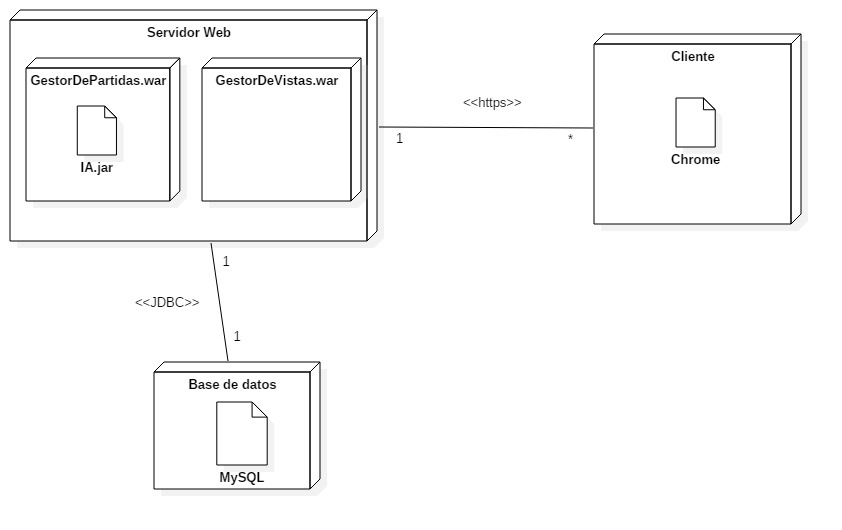
\includegraphics[scale = 0.4]{figuras/despliegue.jpg}
\caption{Diagrama de despliegue}
\label{fig:diagramaDespliegue}
\end{figure}

\subsubsection{Plan de aseguramiento de la calidad}

Uno de los pilares del proyecto es el control de la calidad del software. Para ello el equipo intenta automatizar las tareas a este respecto todo lo posible y apoyarse en los siguientes pilares:
\begin{itemize}
\item{Para garantizar el correcto funcionamiento de los paquetes, clases y funciones generados se realizan diferentes test unitarios. Para las clases cuyos métodos están formados por bucles complejos o varios condicionales se realizan pruebas de caja blanca utilizando la técnica de análisis de caminos. Para el resto de métodos no triviales se realizan pruebas de caja negra con clases de equivalencias y análisis de valores del límite para aquellos métodos que resuelven problemas con valores pertenecientes a unos rangos concretos. Para las pruebas unitarias en Java y Javascript, se utilizan JUnit y unit.js respectivamente. Estas pruebas deben ser satisfactorias antes de cada commit para, adicionalmente, dar un mínimo de garantías de funcionamiento correcto del código que se almacena en el repositorio.\\ Además, uno de los integrantes del equipo se va a dedicar a realizar pruebas manuales jugando varias partidas en un simulador en las fases iniciales del proyecto y en el sistema real una vez implementado.}
\item{Para la integración de los diferentes módulos entre sí, se realizan test de integración.}
\item{Como guías de estilo, se utilizan las de Google para Java, Javascript, HTML y CSS. En el caso de que a lo largo del desarrollo se introduzca algún lenguaje nuevo, los responsables de equipo y el director consensúan el uso de una guía de uso concreta. En caso de no existir una, se crea un documento con directivas importantes a seguir al utilizar ese lenguaje.}
\item{Para representar y especificar el sistema tanto dentro como fuera de la organización, se utiliza el estándar UML, agilizando y concretando la comunicación entre equipos, evitando errores causados por una mala comprensión de la arquitectura del sistema.}
\item{Se programa por parejas las partes críticas de la lógica del juego y de la aplicación para reducir el número de errores y mejorar la calidad del código en general.}
\item{Cada 30 días se realiza una revisión de requisitos de la aplicación en la que se especifican los requisitos cumplidos y los pendientes.}
% \item  \textbf{Estándares de código y otros (se pueden definir guías para la documentación de diseño y otros documentos del proyecto).}
%     \item \textbf{ Actividades de control de calidad del código que se realizarán: revisiones de código por pares, revisiones de requisitos o diagramas UML por pares, tipos de tests automáticos o manuales que se llevarán a cabo.}
\end{itemize}
\subsubsection{Calendario del proyecto y división del trabajo}
	\begin{figure}[H]
		\hspace{-3cm}
		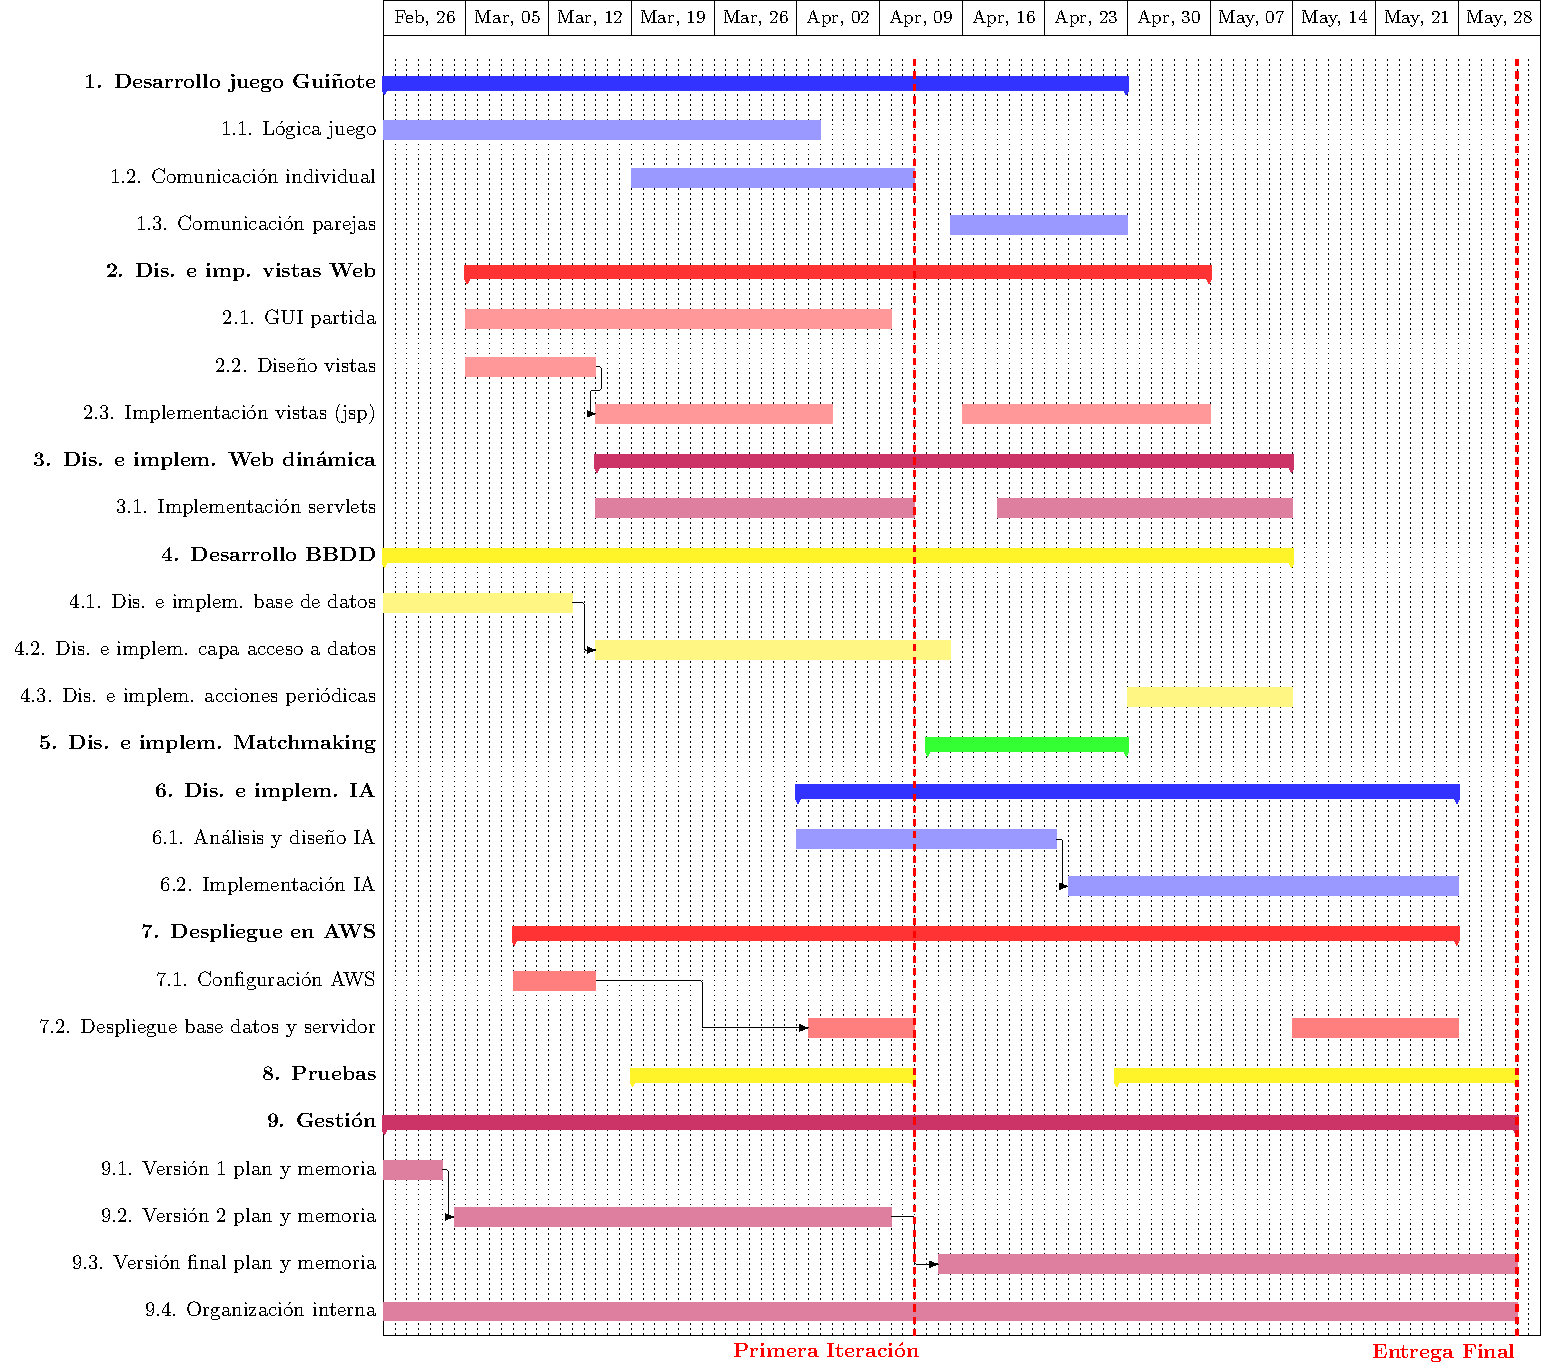
\includegraphics[scale=0.8]{figuras/gantt.pdf}
		\caption{Diagrama de Gantt}
	\end{figure}
% \begin{itemize}
%     \item\textbf{ Diagrama de Gantt que recoja las tareas a realizar. Tened en cuenta que trabajáis con dos iteraciones y por tanto que hay una entrega intermedia y una final, y reflejarlo en este diagrama. Tened en cuenta que es normal que lo tengáis que actualizar conforme avance el proyecto (cuándo y cómo establezcáis en la sección 3.1.2).}
%      \item \textbf{Debe quedar claro qué requisitos van a estar completados en la primera iteración y cuáles en la segunda. Es posible que para la primera iteración no se planifique completar ningún requisito, pero en ese caso tiene que planificarse qué se hará y que faltará por hacer para cada requisito.}
%     \item \textbf{División del trabajo en partes (los módulos del software a desarrollar, pero también  la documentación, el diseño gráfico, instalaciones o despliegues, pruebas manuales etc.) y reparto de los mismos entre el equipo de desarrollo, al menos a alto nivel (el reparto de labores concretas en el día a día no se detalla aquí, pero hay que explicar bajo qué criterios y quién/cómo se hace en la sección 3.1.2). Debe haber una correspondencia con las tareas que aparecen en el diagrama de Gantt (que no necesariamente tiene que ser una relación 1 a 1).}
%      \item \textbf{Verificar que esta división del trabajo cubre todos los requisitos}
% \end{itemize}

Como se observa en el diagrama, el proyecto está dividido en dos iteraciones, con sus correspondientes demostraciones al cliente del avance del proyecto. La primera iteración finaliza la semana del 9 de abril y la segunda, que se corresponde con la entrega final, el 1 de junio.\\

%TODO: terminar esta sección cuando marius acabe los requisitos (cambiando los numeros o quizas hablando de bloques de requisitos)
\textbf{Primera iteración}

En la primera iteración se presenta una partida funcional individual, así como la página web con las vistas de las pantallas de login y perfil de usuario. También esta disponible el modo espectador. La inteligencia artificial está analizada pero no implementada todavía.

En concreto, los requisitos funcionales 2-6, 9-10 y los requisitos no funcionales 1-2 está cubiertos completamente. Además, el requisito funcional 1 está cubierto en cuanto a las partidas individuales, pero queda la implementación de las partidas por parejas. El requisito funcional 13 está cubierto parcialmente, ya que los turnos tienen un periodo de tiempo establecido, acabando la partida si el jugador no realiza movimiento, pero el sistema de puntuaciones no esta implementado.
De la misma forma, relativo a los requisitos funcionales 14 y 17, se puede abandonar la partida manualmente pero todavía no hay penalización de puntuaciones. Finalmente, el requisito funcional 24 correspondiente al desarrollo de la inteligencia artificial, queda cubierto solo parcialmente, en lo que respecta a análisis y representación del problema pero no la implementación e integración con el resto del sistema.\\

\textbf{Segunda iteración}

En la segunda iteración o entrega final, se presenta al cliente el sistema con todas las características especificadas totalmente funcionales. Se añaden a las funcionalidades de la primera iteración todas las correspondientes a las puntuaciones, las ligas y los torneos (así como su programación automática), el sistema de matchmaking, la tienda, el panel de administración y la inteligencia artificial.

En concreto, se cubren por completo los requisitos funcionales 1, 7-8, 11-24 y los no funcionales 3-7.


\subsubsection*{División del trabajo}
\label{repartotrabajo}
A continuación, se detalla una división del proyecto en bloques, con el correspondiente equipo o equipos de los descritos en la sección \ref{organiz} que los lleva a cabo. Además, se incluye la lista de requisitos (especificados en el apartado \ref{requisitos}) que quedan cubiertos en cada uno de estos bloques para garantizar que se satisfacen todos ellos.
%TODO: terminar con los requisitos

\begin{table}[H]
\label{divisionTrabajo}
\hspace{-0.8cm}
\begin{tabular}{|l|c|l|}
\hline
\multicolumn{1}{|c|}{\textbf{Bloque}}                          & \textbf{Equipo} & \multicolumn{1}{c|}{\textbf{Requisitos}}                                                                       \\ \hline
Desarrollo de la interfaz del guiñote                 & 1      & \begin{tabular}[c]{@{}l@{}}\small{RF: 1,6}\\ \small{RNF: 2}\end{tabular}                                              \\ \hline
Desarrollo de la lógica de juego del guiñote          & 4      & \begin{tabular}[c]{@{}l@{}}\small{RF: 1}\\ \small{RNF: -}\end{tabular}                                                \\ \hline
Diseño e implementación de vistas web                 & 1      & \begin{tabular}[c]{@{}l@{}}\small{RF: 2,4,6,7,8,9,11,15,18,19,20,21}\\ \small{RNF: 2}\end{tabular}                    \\ \hline
Implementación de la web dinámica                     & 4      & \begin{tabular}[c]{@{}l@{}}\small{RF: 1,6,12,13,14,16,17}\\ \small{RNF: 3,5}\end{tabular}                             \\ \hline
Diseño e implementación de las comunicaciones         & 1      & \begin{tabular}[c]{@{}l@{}}\small{RF: 1,3,4,12}\\ \small{RNF: 1,2}\end{tabular}                                       \\ \hline
Desarrollo de la base de datos                        & 2      & \begin{tabular}[c]{@{}l@{}} \small{RF: 2,4,7,9,11,13,14,15,16,17,18,19,20,22,23}\\ \small{RNF: 1,3,4,5,6}\end{tabular} \\ \hline
Diseño e implementación de la Inteligencia Artificial & 3      & \begin{tabular}[c]{@{}l@{}}\small{RF: 24}\\ \small{RNF: -}\end{tabular}                                               \\ \hline
Despliegue                                            & 2      & \begin{tabular}[c]{@{}l@{}}\small{RF: 10}\\ \small{RNF: 1}\end{tabular}                                               \\ \hline
\end{tabular}
\caption{Tabla de división del trabajo}
\end{table}

\section{Análisis y diseño del sistema}
\label{analisis}
\subsection{Análisis de requisitos}
\label{requisitos}

\begin{table}[H]
\centering
\begin{tabular}{|c|p{12cm}|}
\hline
\multicolumn{2}{|c|}{GUIÑOTE} \\ \hline
RF-1 &  El sistema permite a los usuarios jugar al guiñote en modo uno contra uno y dos contra dos. \\ \hline
RF-2 & El sistema almacena un historial de partidas jugadas por el usuario y permite visualizar estadísticas de las partidas jugadas. \\ \hline
RF-3 & El jugador, en mitad de una partida, puede desconectarse y   volver a conectarse desde cualquier dispositivo siempre que no sea su turno o, en caso de serlo, no agote su tiempo de turno. \\ \hline
RF-4 & El sistema requiere que los usuarios se registren con su correo electrónico o Facebook para poder acceder a los servicios que ofrece. \\ \hline
RF-5 & El jugador puede seleccionar si desea jugar una partida pública o privada. \\ \hline
RF-6 & Los usuarios pueden elegir una partida pública en curso y unirse a ella como espectadores. \\ \hline
RF-7 & El sistema cuenta con una divisa virtual que se consigue al iniciar sesión por primera vez, ganando torneos, partidas, ascensos a otra liga, etc. \\ \hline
RF-8 & El sistema consta de un panel de administración al cual se pueden conectar solamente los usuarios definidos como administradores con anterioridad. \\ \hline
RF-9 & El sistema permite al usuario administrar sus datos personales almacenados en el sistema: nombre de usuario, avatar, correo electrónico. \\ \hline
RF-10 & El usuario debe conectarse utilizando el navegador web Google Chrome para garantizar el correcto funcionamiento del sistema. \\ \hline
RF-24 & El usuario puede jugar contra un agente de inteligencia artificial, únicamente en el modo uno contra uno.  \\ \hline
RNF-1 & El sistema garantiza la seguridad de la información de los usuarios. \\ \hline
RNF-2 & El sistema permite la conexión desde diferentes dispositivos. La aplicación es responsive por lo que se muestra de forma diferente para cada uno de los diferentes tamaños de pantalla. \\ \hline
RNF-3 & El sistema tarda menos de 20 segundos en encontrar partida aleatoria en caso de que haya un número de jugadores suficientes esperando para iniciar partida con las mismas características. \\ \hline
\end{tabular}
\caption{Requisitos relacionados con la jugabilidad y el usuario}
\label{tabla-usuario}
\end{table}


\begin{table}[H]
\centering
\begin{tabular}{|c|p{12cm}|}
\hline
\multicolumn{2}{|c|}{LIGAS} \\ \hline
RF-11 & Los jugadores tienen asociada una puntuación que varía en función de las partidas ganadas o perdidas. Dependiendo de ésta, pertenecerán a una u otra liga. \\ \hline
RF-12 & El sistema primero intenta emparejar a los jugadores de la misma liga. Si no es posible, los empareja con los de la liga más cercana a la suya. \\ \hline
RF-13 & Si el usuario no realiza ninguna acción durante su turno, la partida se termina y él recibe una penalización de puntuación. El turno es un periodo de tiempo preestablecido. \\ \hline
RF-14 & El sistema permite que los jugadores abandonen manualmente una partida de liga con una penalización asociada a su puntuación. \\ \hline
RNF-4 & Para ascender a una liga superior el jugador debe haber ganado muchas partidas. \\ \hline
\end{tabular}
\caption{Requisitos de las ligas}
\label{tabla-ligas}
\end{table}

\begin{table}[H]
\centering
\begin{tabular}{|c|p{12cm}|}
\hline
\multicolumn{2}{|c|}{TORNEOS} \\ \hline
RF-15 & El sistema permite a los usuarios inscribirse y participar en torneos. Los torneos son competiciones con eliminatorias directas a una partida única, en las cuales se pasa a la siguiente ronda ganando la partida. \\ \hline
RF-16 & Por cada ronda del torneo ganada el jugador recibe una puntuación proporcional a la ronda del torneo siendo la mayor bonificación la del ganador del torneo. \\ \hline
RF-17 & Los jugadores que abandonen una partida de un torneo son descalificados con una penalización asociada a su puntuación. \\ \hline
RF-18 & El administrador puede programar la creación automática de torneos ya sean puntuales o periódicos, especificando un momento de inicio y unos premios determinados. \\ \hline
RF-19 & El administrador puede modificar y eliminar torneos que aún no estén en curso. \\ \hline
RNF-5 & La puntuación recibida en cada fase por ganar una partida es mucho mayor que la recibida en una partida de liga y el doble que la de la fase anterior del mismo torneo. La puntuación para el campeón y el subcampeón es mucho más grande que la de los otros participantes. \\ \hline
RNF-6 & Los torneos programados inicialmente son semanales. \\ \hline
\end{tabular}
\caption{Requisitos de los torneos}
\label{tabla-torneo}
\end{table}

\begin{table}[H]
\centering
\label{tabla-tienda}
\begin{tabular}{|c|p{12cm}|}
\hline
\multicolumn{2}{|c|}{TIENDA} \\ \hline
RF-20 & El sistema posee una tienda para personalizar el tablero de juego, las barajas y el avatar, que inicialmente consta de 3 barajas, 3 tableros y 20 avatares diferentes. \\ \hline
RF-21 & El administrador de la aplicación puede añadir artículos nuevos a la tienda y modificar el   precio de los existentes \\ \hline
RF-22 & Los artículos de la tienda se desbloquean en función de la liga más alta en la que ha participado el usuario en algún momento. \\ \hline
RF-23 & Los artículos se compran con la divisa virtual que el usuario tiene acumuladas. \\ \hline
RNF-7 & El valor en divisas virtuales de las barajas es más mayor que el de los tableros. El precio de los avatares varía para cada uno de ellos y para conseguirlos el jugador debe haber ganado muchas partidas. \\ \hline
\end{tabular}
\caption{Requisitos de la tienda}
\end{table}


\subsection{Diseño del sistema}
Se ha decidido implementar una aplicación web de 3 capas porque como se accede desde el navegador para hacer un cambio en la interfaz no hace falta una actualización en cada nodo cliente, siempre que la nueva interfaz sea compatible con Google Chrome 64 o posteriores. Además, como el modelo se aloja en un servidor distinto al de la base datos cualquier cambio en una de las partes no afecta al resto del sistema ya que se comunica mediante una interfaz bien definida al comienzo del proyecto. 
Otra ventaja de las aplicaciones en tres capas es que es muy fácil encontrar documentación y ejemplos de otras aplicaciones parecidas en internet ya que hoy en día son las más utilizadas. \\
No se ha elegido un modelo de aplicación de 4 capas porque resulta un inconveniente que la interfaz se ejecute en un servidor central ya que sería un cuello de botella importante para el sistema dado que gran parte del tiempo de ejecución del sistema corresponde a la interfaz. \\

La distribución de las diferentes partes se puede apreciar en el diagrama de componentes de la figura \ref{fig:diagramaComponentes}

\begin{figure}[H]
\centering
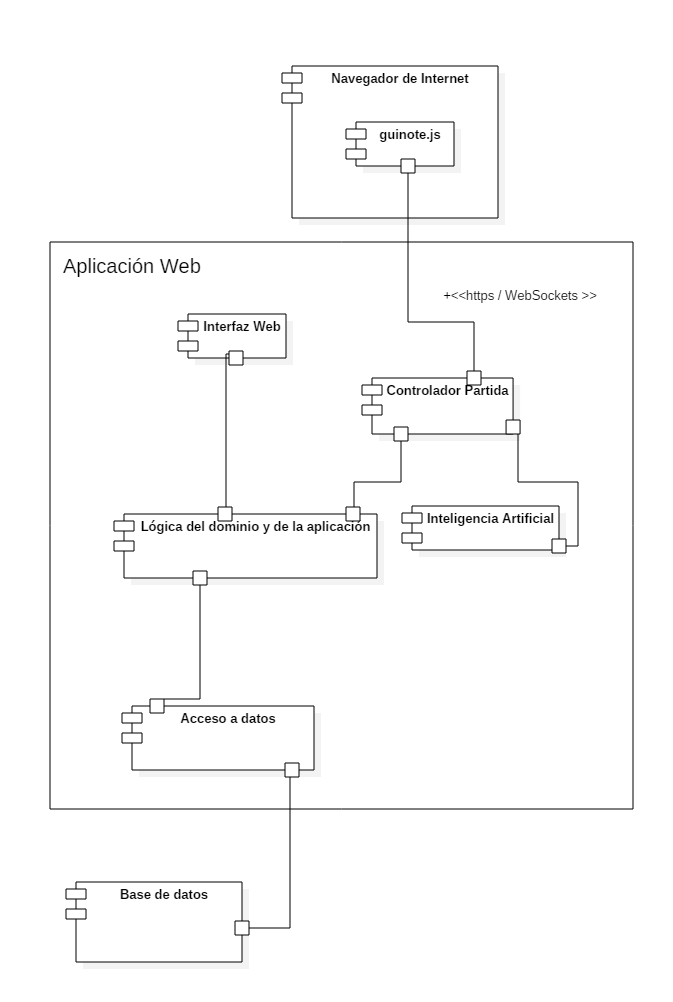
\includegraphics[scale = 0.5]{figuras/diagramaComponentes.png}
\caption{Diagrama de componentes donde se refleja la distribución del sistema}
\label{fig:diagramaComponentes}
\end{figure}

\subsubsection{Interfaz}
La interfaz se ha desarrollado utilizando la herramienta Phaser, basada en JavaScript. Se ha implementado de manera que sea fácilmente modificable ya que a lo largo de la producción del software se han de introducir cambios, por lo que se han parametrizado la mayoría de las funciones en medida de lo posible.

Una de las principales decisiones de diseño que se han tenido que llevar a cabo es como representar a cada jugador. Se ha hecho de manera que cada jugador tiene su posición como referencia y la interfaz es capaz de representar al resto en función de éste. Como hay un máximo de 4 jugadores, la interfaz toma cada posición como un rol,  teniendo todos los roles los mismos parámetros simulando un patrón de diseño Strategy, para facilitar la integración. El diagrama de clases de la figura \ref{fig:clasesInterfazJuego} muestra la implementación de la interfaz. Aunque en JavaScript no haya clases como tal, se ha aprovechado la sintaxis UML para visualizar las diferentes partes.

\begin{figure}
  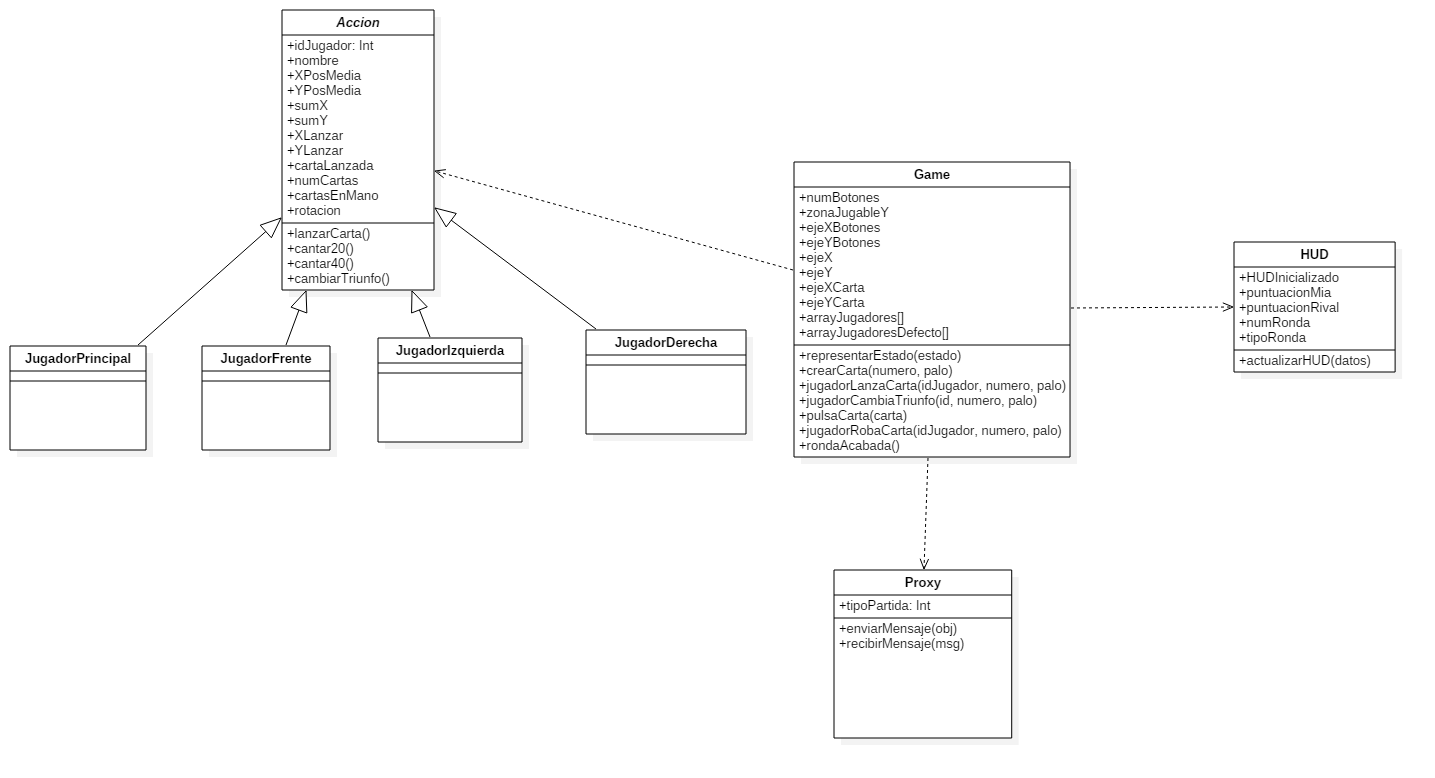
\includegraphics[width=\linewidth]{figuras/clasesInterfazJuego.png}
  \caption{Diagrama de clases de la interfaz de juego}
  \label{fig:clasesInterfazJuego}
\end{figure}

Otra decisión de diseño que sobre la que se ha reflexionado ha sido acerca de la comunicación entre la interfaz y el controlador de la partida. La tecnología que se ha escogido han sido WebSockets como se ha dicho previamente. Dicha tecnología permite únicamente comunicarse a través del paso de mensajes, por lo que se ha decidido que los mensajes sean en formato JSON para que sean fácilmente legibles para ambos extremos de la comunicación.

La aplicación web que no se corresponda con la parte jugable, es decir, el perfil del usuario, la vista del historial de partidas, ligas, torneos, etc. se implementa con JSP y servlets. Se puede observar el mapa de navegación inicial de la aplicación en la figura \ref{fig:mapaDeNavegacion}.

\begin{figure}
  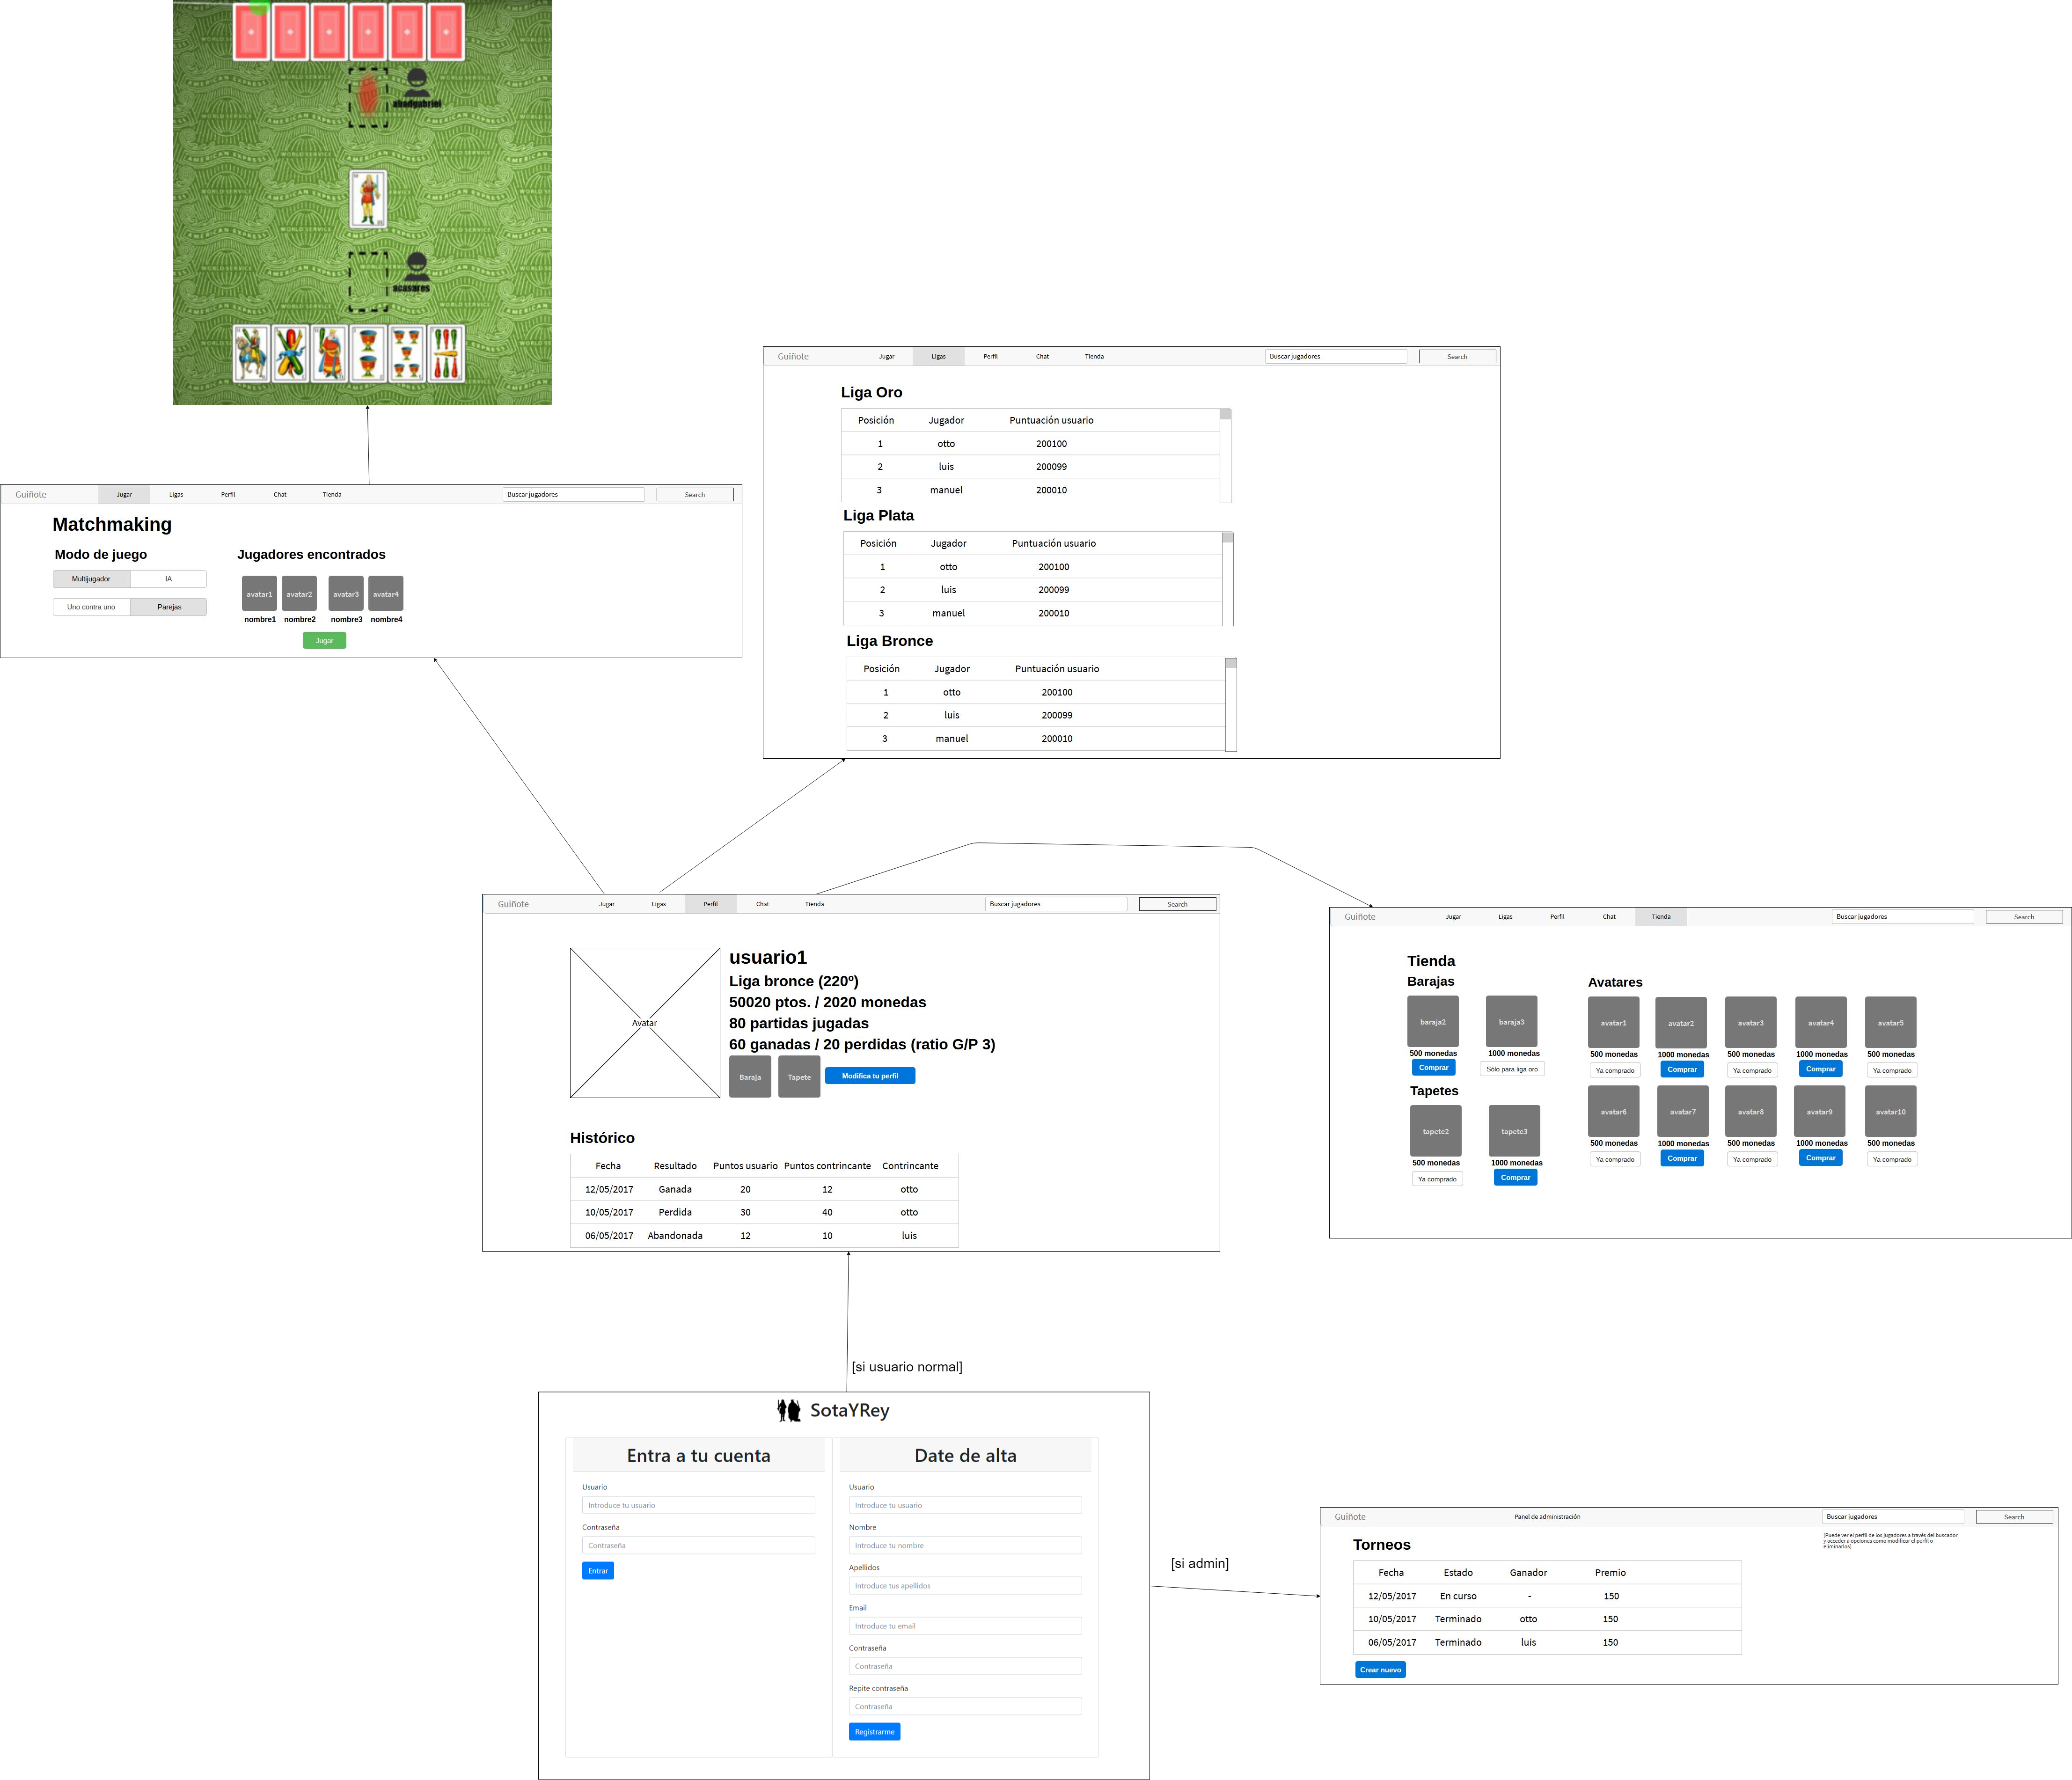
\includegraphics[width=\linewidth]{figuras/mapaNavegacion.png}
  \caption{Mapa de navegación}
  \label{fig:mapaDeNavegacion}
  \ref{fig:mapaNavegacion}
\end{figure}

Una vez se ha desarrollado el sistema, con todas las vistas ya implementadas, el mapa de navegación resultate se observa en la figura \ref{fig:mapaDeNavegacionFinal}.

\begin{figure}
  \includegraphics[width=\linewidth]{figuras/mapNavFinal.png}
  \caption{Mapa de navegación final}
  \label{fig:mapaDeNavegacionFinal}
  \ref{fig:mapaNavegacion}
\end{figure}

\subsubsection{Lógica y BackEnd}

Para la implementación de la lógica del juego se ha análizado el dominio del problema y se ha realizado un primer diseño de clases de análisis. Posteriormente se ha implementado objeto a objeto el diseño inicial y al mismo tiempo actualizando el diagrama de clases.

\begin{figure}[H]
\hspace{-1cm}
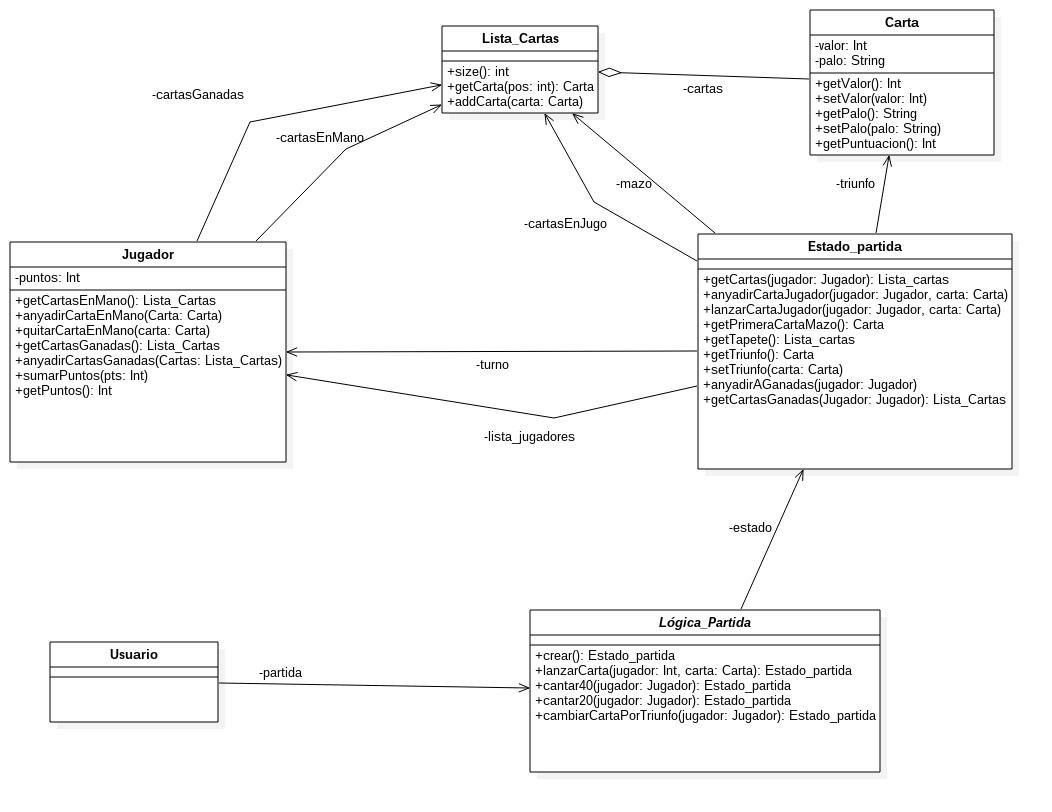
\includegraphics[scale = 0.5]{figuras/logica_juego/diagramaClasesDisenyo.png}
\caption{Diagrama de clases en la fase de análisis del problema}
\label{fig:diagramaClasesLogicaJuegoInicial}
\end{figure}

\begin{figure}[H]
\hspace{-2cm}
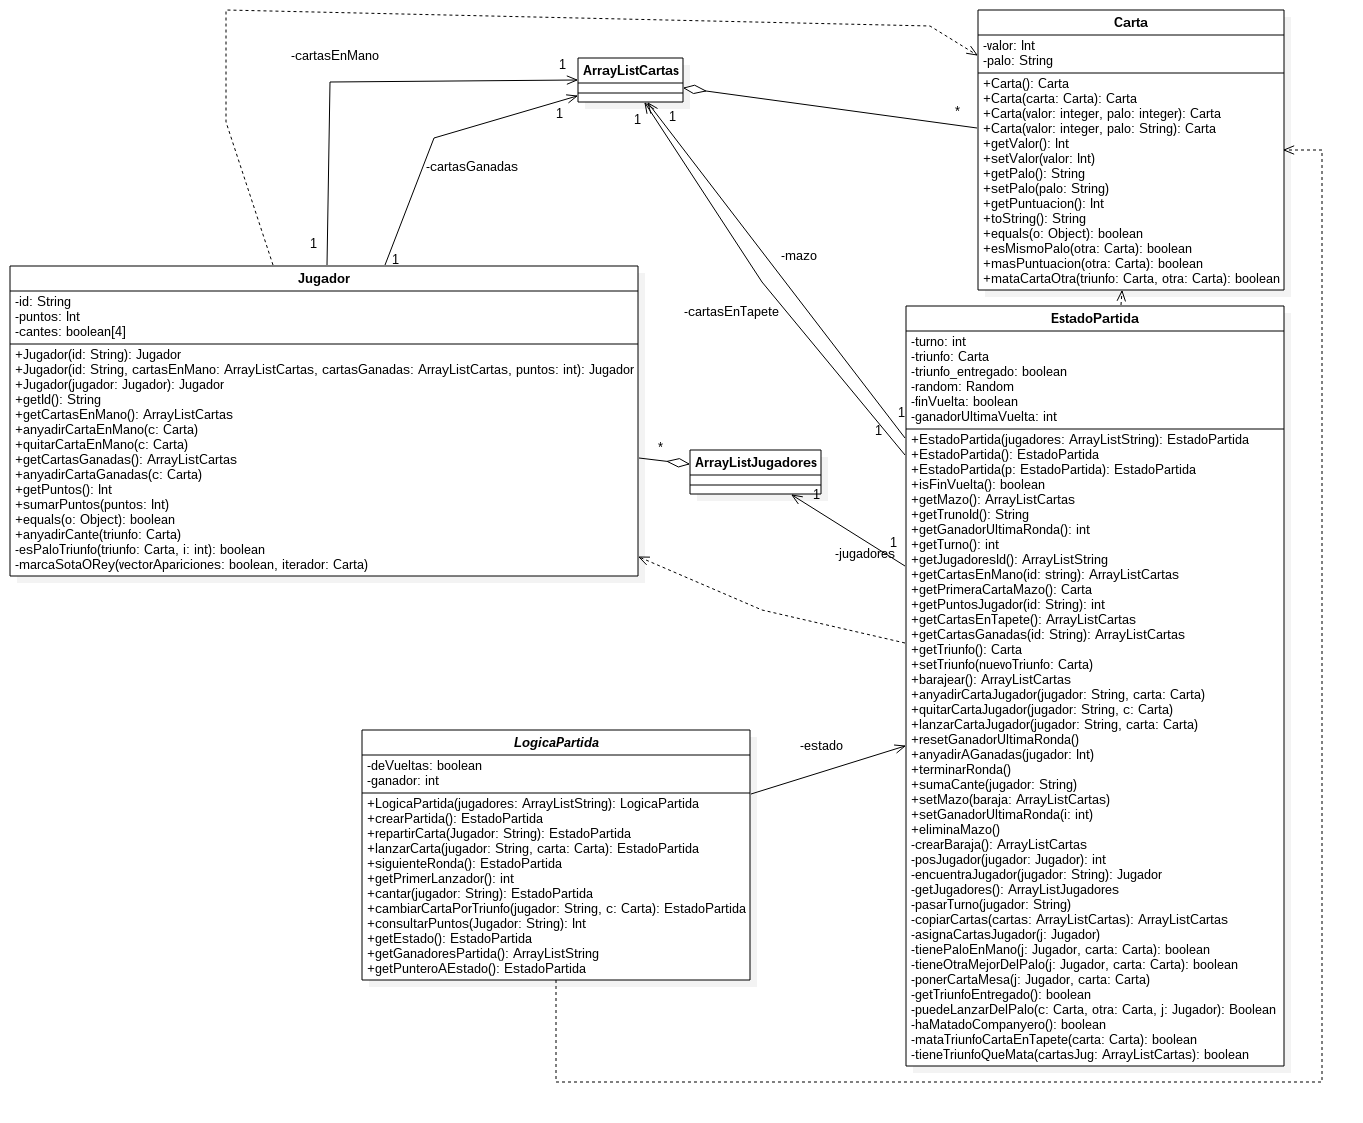
\includegraphics[scale = 0.4]{figuras/logica_juego/diagramaClasesImplementacion.png}
\caption{Diagrama de clases final}
\label{fig:diagramaClasesLogicaJuegoFinal}
\end{figure}


\subsubsection{Base de Datos}
El primer paso en el diseño de la base de datos fue plantear el esquema entidad relación como esquema conceptual del problema. Una vez diseñado el paso a un esquema relacional fue sencillo.

\begin{figure}[H]
\centering
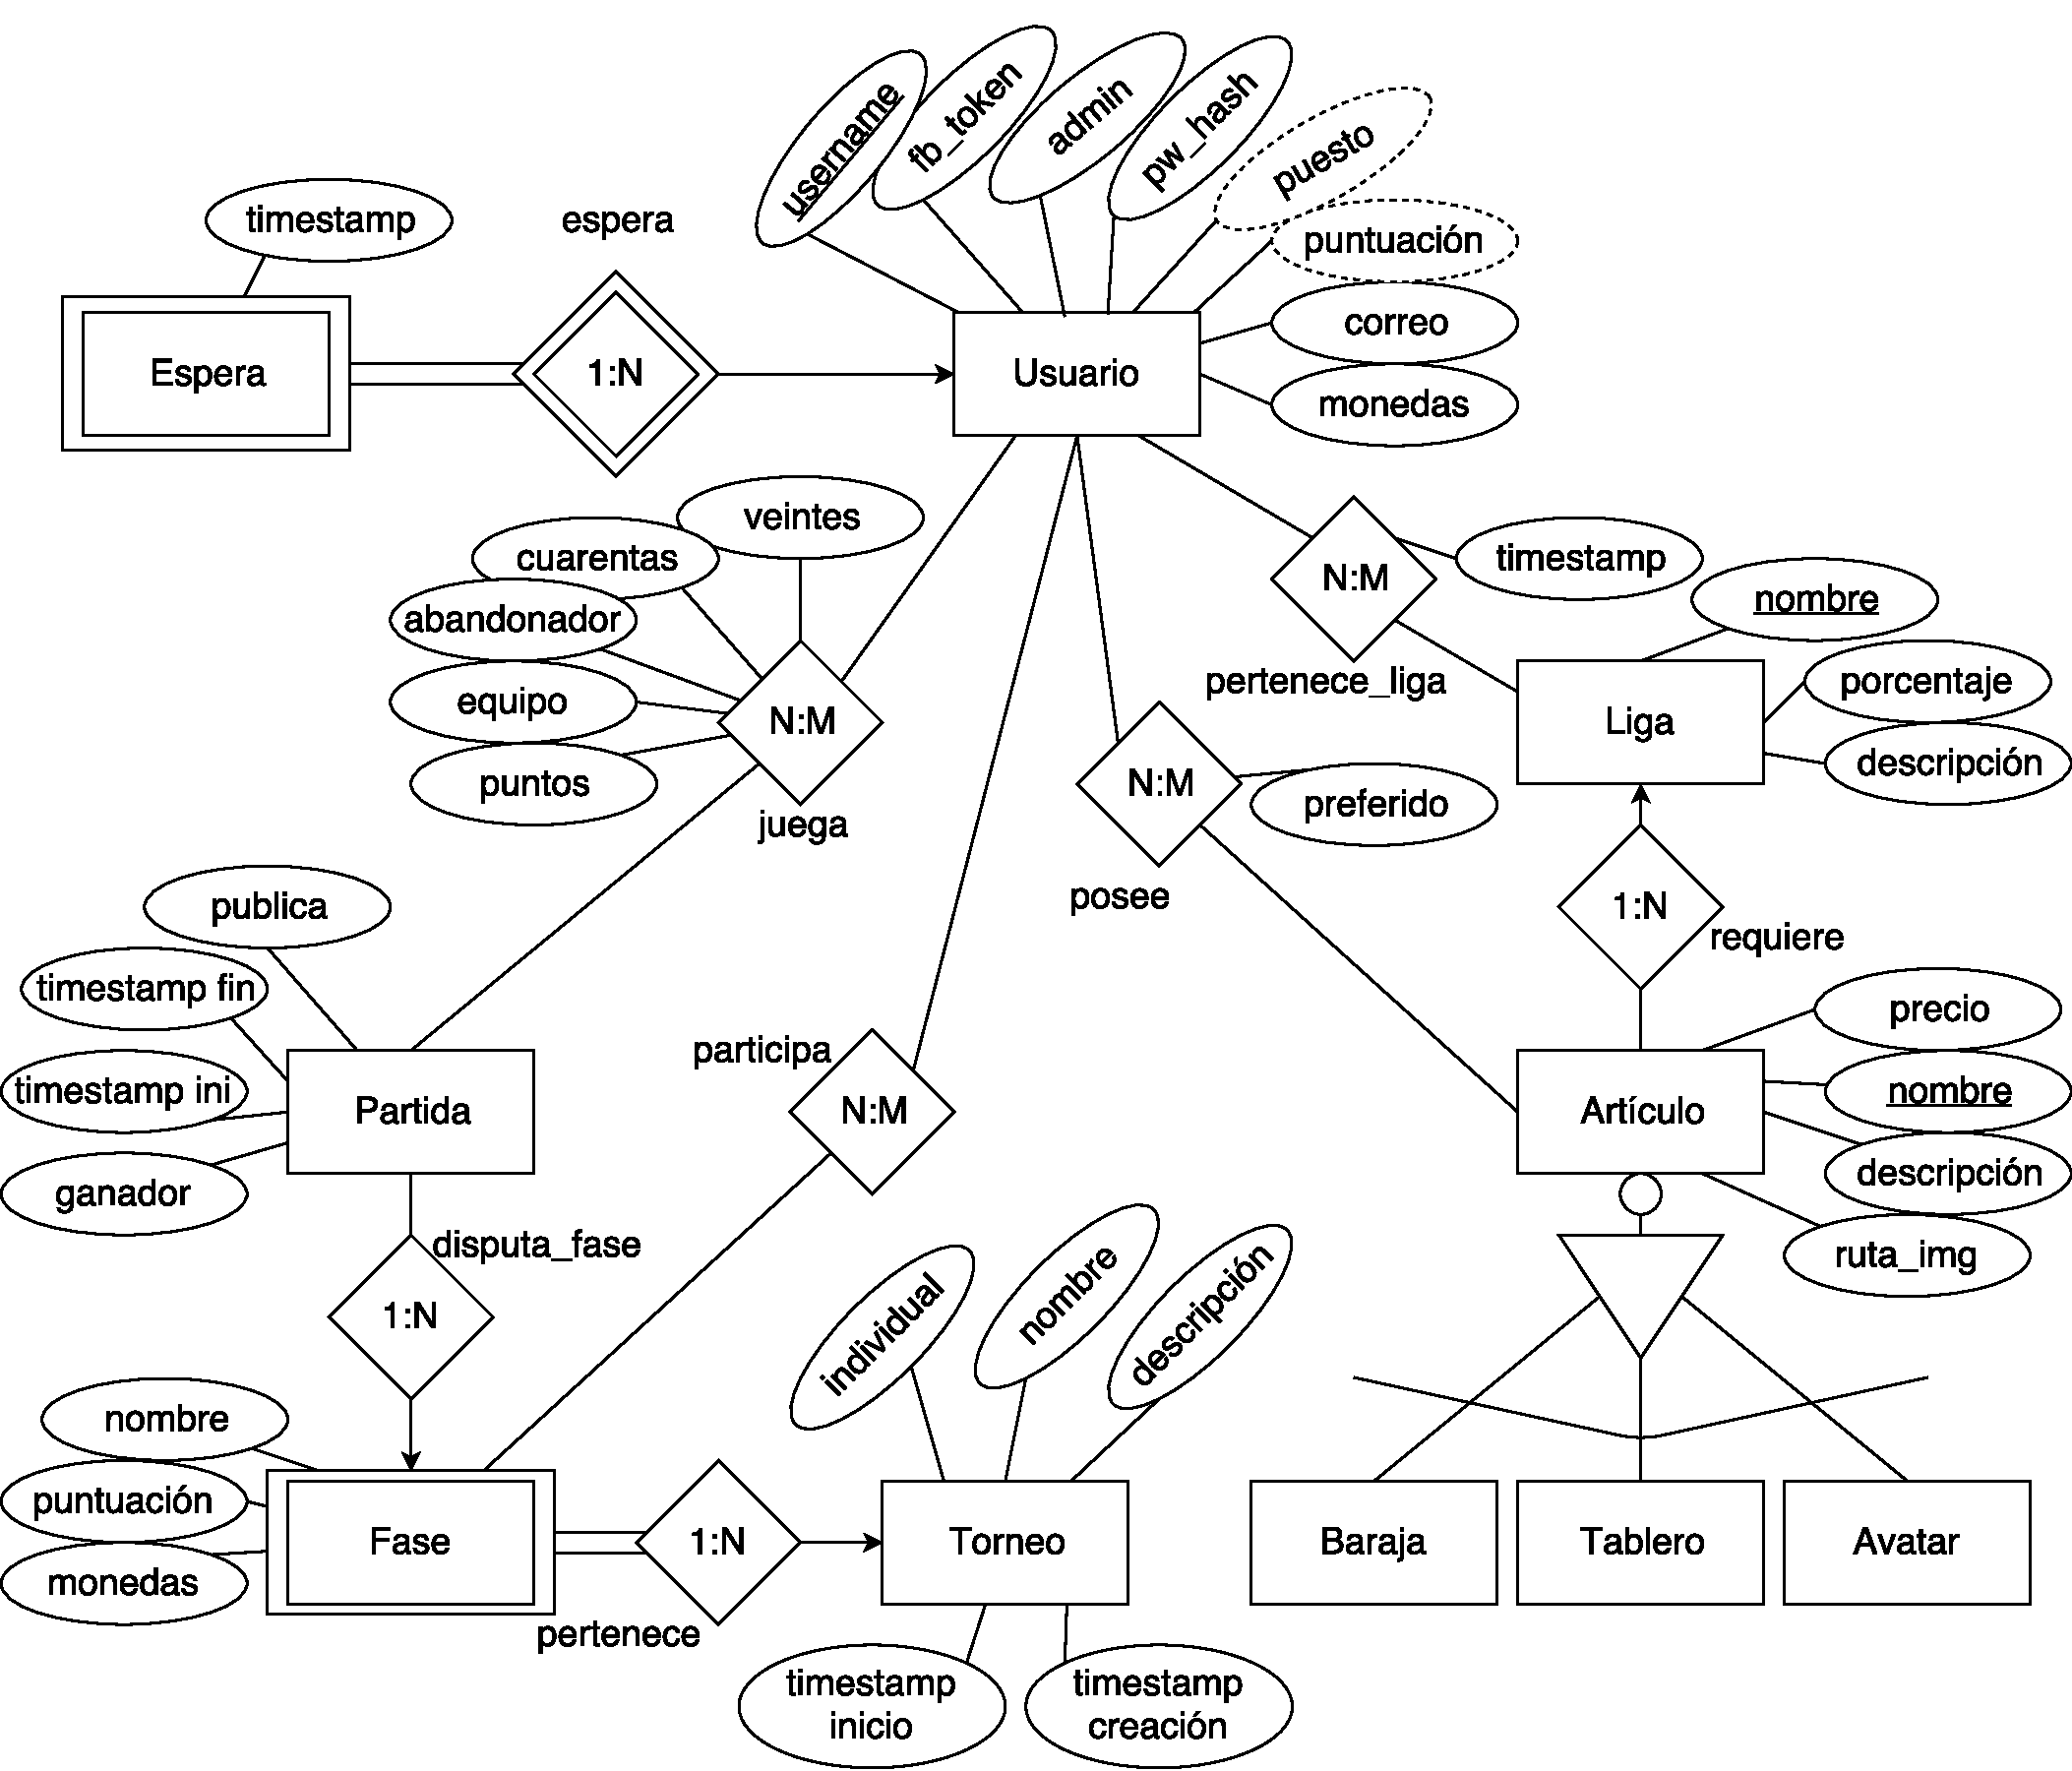
\includegraphics[scale = 0.5]{figuras/base_datos/diagrama-conceptual.pdf}
\caption{Esquema Conceptual}
\label{fig:diagramaConceptual}
\end{figure}

Antes de llegar al esquema actual se plantearon otras posibilidades, primeramente por una falta de claridad entre los datos que debían ser persistentes y los que no. En un primer momento se creó una entidad Espera, débil respecto a un Usuario que representaba que un usuario estaba esperando para encontrar jugadores. Finalmente la entidad no existe y la información de una espera no es almacenada en la base de datos. Las partidas son introducidas en la base cuando se empieza una partida, para así poder tener la información de las partidas en curso. La parte con más dificultad es la relacionada con los torneos. Para representar los torneos existen las fases, entendidas como octavos, cuartos, semifinales... Una partida puede estar ligada a una fase, y la fase pertenece a un torneo. Finalmente los jugadores están relacionados con una fase para poder emparejar jugadores.\\

Para la comunicación del sistema con la base de datos se ha utilizado el patrón DAO (Objeto de Acceso a Datos). Para ello se han implementado una serie de objetos VO que representan la información guardada de forma persistente y unos objetos DAO que abstraen las operaciones con el JDBC mediante métodos de Java. Para mayor seguridad de los datos, todos los posibles usos de la base se realizan a través de una interfaz que proporciona los métodos necesarios además de ofrecer un \textit{pool} de conexiones para aumentar la velocidad de la interacción cuando haya múltiples usuarios.\\

\begin{figure}[H]
\centering
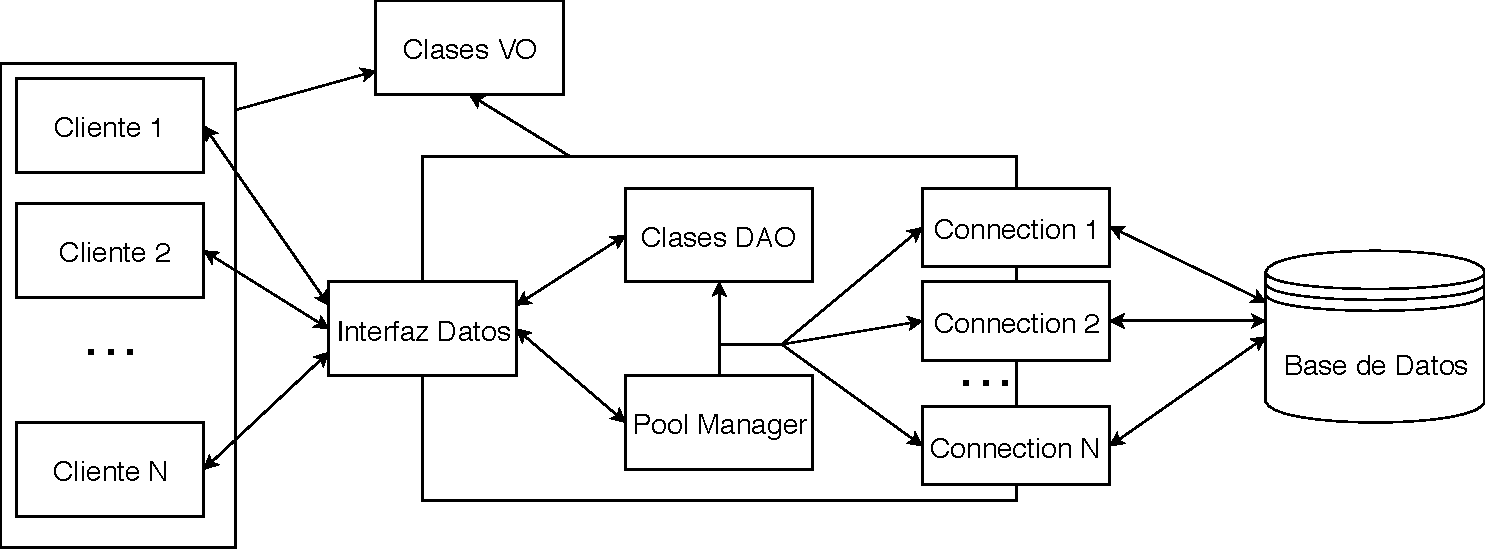
\includegraphics[scale = 0.5]{figuras/base_datos/Componentes.pdf}
\caption{Esquema de la estructura del acceso a datos}
\label{fig:componentesbases}
\end{figure}

Los clientes que usen la base de datos deben realizar todas las operaciones a través de la Interfaz de Datos. La Interfaz utiliza el pool manager para no tener que crear una nueva conexión con cada cliente y poder reutilizarlas. La Interfaz invocará a las clases DAO que utilizaran las conexiones para conectarse finalmente con la base. Las clases VO sirven para representar los objetos de la base en la comunicación entre las clases.\\

Dado el gran número de clases empleado en la implementación del modelo, su representación se ha realizado mediante diferentes diagramas de clases enfocados en las diferentes funcionalidades de la base .
\begin{figure}[H]
\centering
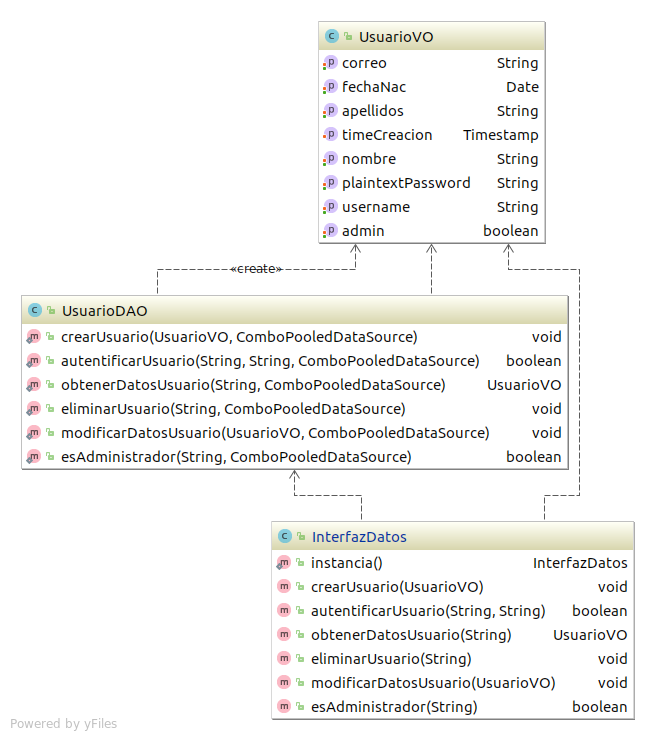
\includegraphics[scale = 0.5]{figuras/base_datos/clasesUsuario.png}
\caption{Diagrama de clases para la funcionalidad de usuario}
\label{fig:diagramaClasesUsuario}
\end{figure}
\begin{figure}[H]
\centering
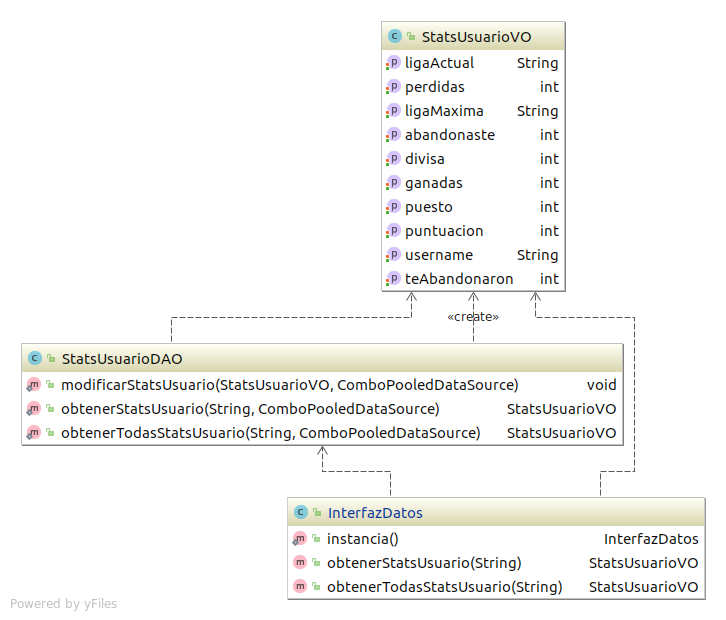
\includegraphics[scale = 0.5]{figuras/base_datos/clasesStats.png}
\caption{Diagrama de clases para la funcionalidad de las estadísticas del usuario}
\label{fig:diagramaClasesStats}
\end{figure}
\begin{figure}[H]
\centering
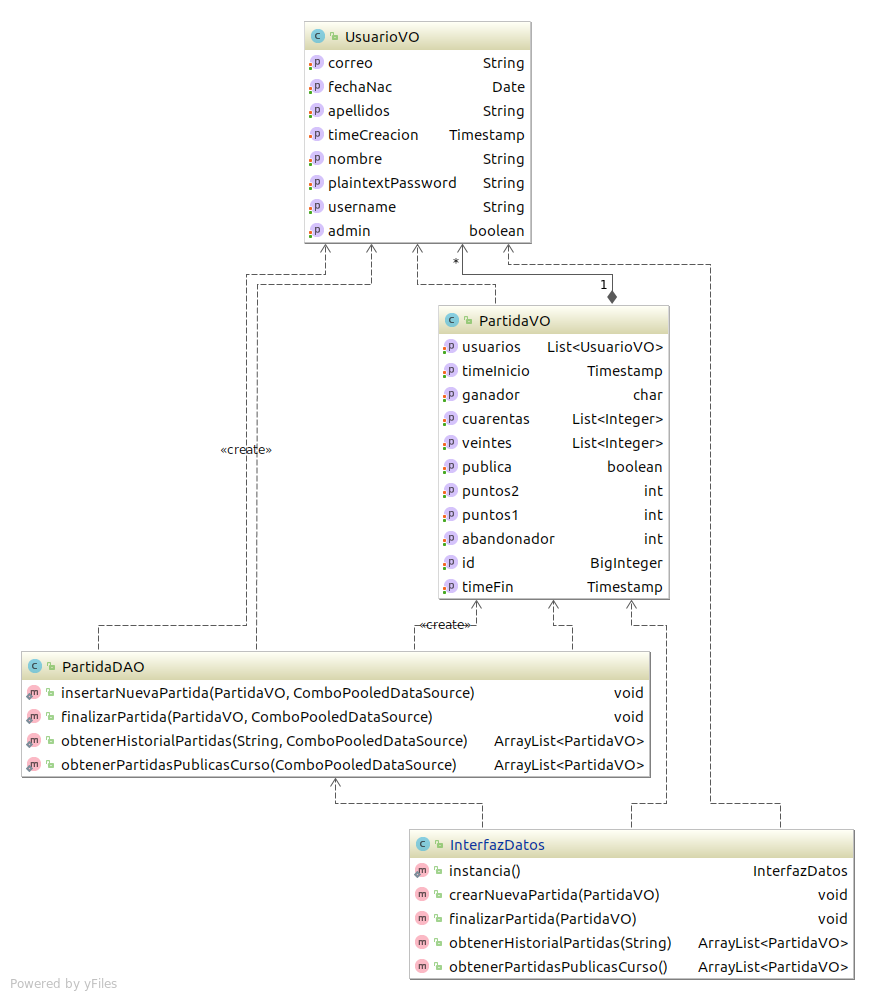
\includegraphics[scale = 0.5]{figuras/base_datos/clasesPartida.png}
\caption{Diagrama de clases para la funcionalidad de partida}
\label{fig:diagramaClasesPartida}
\end{figure}
\begin{figure}[H]
\centering
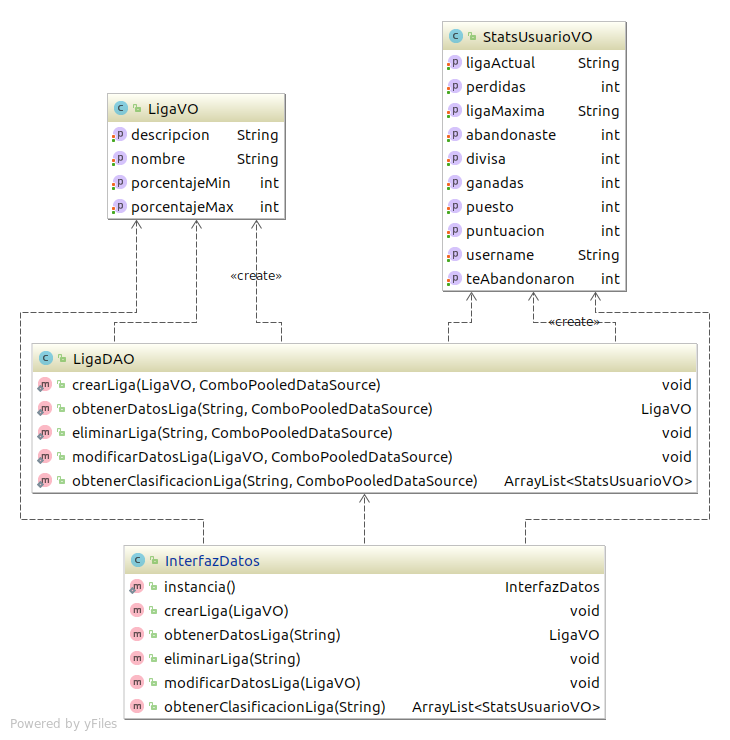
\includegraphics[scale = 0.5]{figuras/base_datos/clasesLiga.png}
\caption{Diagrama de clases para la funcionalidad de liga}
\label{fig:diagramaClasesLiga}
\end{figure}
\begin{figure}[H]
\centering
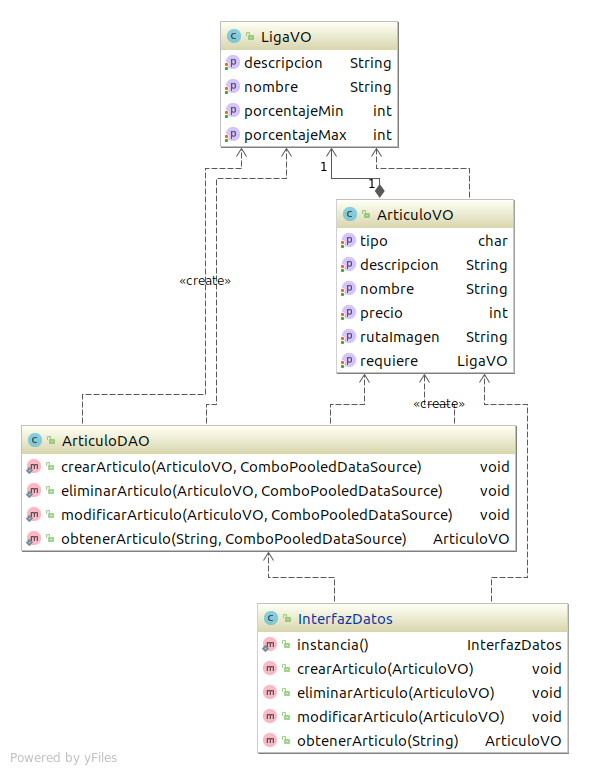
\includegraphics[scale = 0.5]{figuras/base_datos/clasesArticulo.png}
\caption{Diagrama de clases para la funcionalidad de artículo}
\label{fig:diagramaClasesArticulo}
\end{figure}
\begin{figure}[H]
\centering
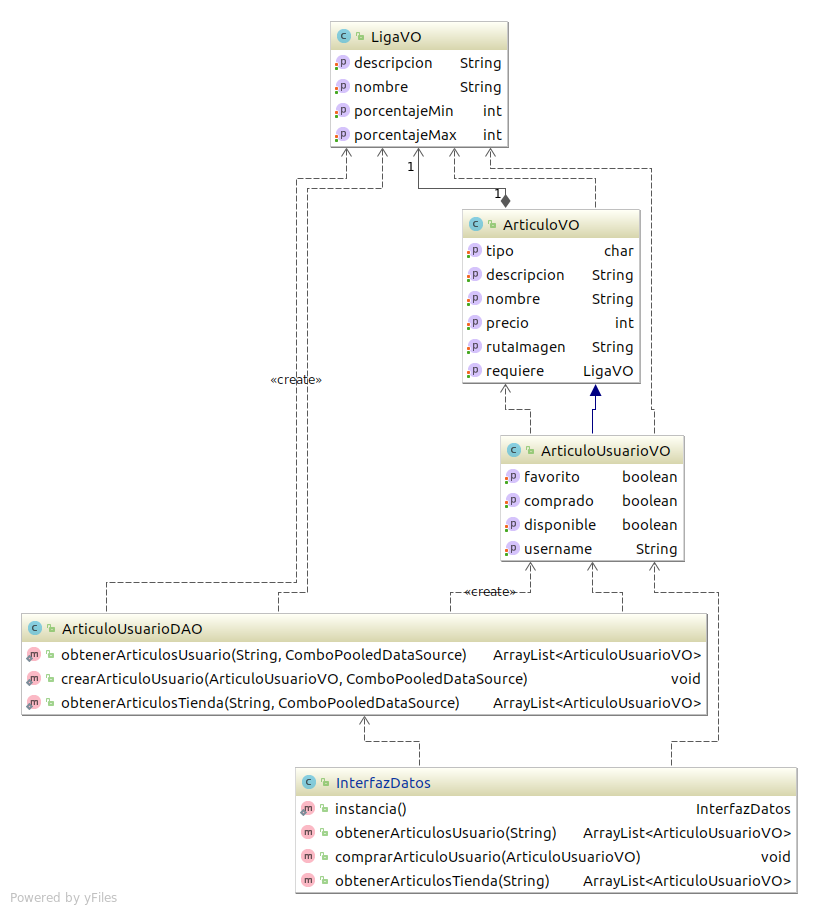
\includegraphics[scale = 0.5]{figuras/base_datos/clasesArticuloUsuario.png}
\caption{Diagrama de clases para la funcionalidad de los artículos de usuario}
\label{fig:diagramaClasesArticuloUsuario}
\end{figure}

\subsubsection{Despliegue}
La aplicación se pone en marcha en un servidor Tomcat, ya que permite la instalación de aplicaciones web en formato .war. Se distinguen dos aplicaciones diferentes: la que da soporte a la lógica de la aplicación y la encargada de coordinar una partida en curso. Ambas se comunican indirectamente a través de la base de datos y están coordinadas. \\
La base de datos es relacional ya que se necesitan muchas consultas de los datos almacenados y para cada partida hay varias inserciones o actualización de los datos almacenados. El sistema gestor de la base de datos va a ser MySQL porque se ahorran costes al ser un SGBD de código abierto y no tener que adquirir una licencia de pago. Además, el equipo cuentan con experiencia en el diseño e implementación de bases de datos utilizando MySQL. \\
La razón por la que no se ha elegido otro SGBD de código abierto son los problemas que presenta RDS Aurora. Otros SGBD como PostgreSQL son más exigentes en recursos y, por lo tanto, el coste es mayor sin repercutir un beneficio real sobre la aplicación ya que se considera que MySQL es más que suficiente para una aplicación de estas características.
Otra alternativa era Oracle pero debido al alto coste de la licencia no se ha escogido. \\
El patrón de diseño utilizado para la comunicación del sistema con la base de datos es \textit{façade} ya que permite dividir el sistema completo en dos o más subsistemas consiguiendo un alto desacoplamiento de la base de datos y el juego. De esta forma, se puede dividir mejor el trabajo de forma independiente entre los equipos para poder llevar a cabo un diseño e implementación top-down.


\subsection{Tecnologías elegidas}
\begin{itemize}
\item \textbf{Interfaz de la partida en el navegador web}. La interfaz del juego consiste en una única pantalla donde los jugadores que participan en la partida en curso se comunican. Se implementa utilizando JavaScript y Phaser. Phaser es un framework para desarrollo de juegos en HTML5 basado en la tecnología JavaScript.  \\ Se ha decidido utilizar JavaScript por la sencillez a la hora de ser visualizado en un navegador y se incorpora a la perfección con HTML5. Se ha barajado la posibilidad de utilizar Flash pero se descarta por estar obsoleta y porque algunos navegadores ya no lo soportan. También se podría haber utilizado Unity pero no se ha llevado a cabo por tener una curva de aprendizaje muy complicada.
\item \textbf{Capa de comunicación de la partida}. Es el servicio que está por debajo de la partida encargado de notificar las acciones de los jugadores al resto. Además comprueba que el transcurso de la partida es correcto, como si de un coordinador se tratara. Se utiliza lenguaje Java, ya que es un servicio Web e irá desplegado a través de un archivo .war. Además, facilita la comunicación con la tecnología WebSockets, que es la que se ha escogido para comunicar en tiempo real el navegador con el controlador. Se ha decidido WebSockets por tener una curva de aprendizaje sencilla ya que se utilizará para enviar mensajes desde el navegador al controlador. Se integra perfectamente con Java. \\
Se ha descartado utilizar Sockets.io ya que va ligado a Node.js, que es una tecnología más novedosa pero que el equipo desconoce por completo, aprenderla supone un número de horas extras y se desconoce si es una tecnologia viable para la aplicación a desarrollar.
\item \textbf{Interfaz Web}. Se implementa en HTML 5 y se utiliza  JSP y Servlets para la generación de contenido dinámico y procesamiento de formularios, respectivamente. Se trata de una tecnología poco actual pero de la cuál el equipo de desarrollo tiene cierta experiencia, por lo que se asegura la calidad del servicio.
\item \textbf{Lógica y dominio de la aplicación}. Implementado en Java para favorecer la interoperabilidad con la interfaz web.
\item \textbf{Acceso a los datos}. Se utilizan objetos de tipo implementados en Java. De esta manera se cumple el patrón "Modelo - Vista - Controlador".
\item \textbf{Base de datos}. Se utiliza un Sistema Gestor de Bases de Datos relacional, ya que la principales consultas que se hacen son de tipo JOIN. Se ha decidido utilizar MySQL ya que es un sistema que el equipo domina. La desventaja es que es poco eficiente en comparación con otros como Oracle, pero para el número de usuarios que tendrá la aplicación es suficiente con dicho gestor.
\end{itemize}



%\begin{itemize}
%\item  DIAGRAMA DE DESPLIEGUE DE LA APPLICACIÓN WEB EN 3 CAPAS
%\item \textbf{Diagramas arquitecturales (de módulos, de componentes y conectores, de distribución), patrones de diseño y estilos arquitecturales que se aplicarán. Las interfaces (de módulos y de componentes) son especialmente importantes. También lo son los protocolos de comunicación entre componentes.}
%\item \textbf{Tecnologías elegidas (lenguajes de programación, componentes que se integrarán, API web externas con las que se conectará etc.)--ya está--.}

%\item \textbf{Otros aspectos técnicos de interés (p.ej. si hay base de datos si va a ser SQL,  si algunas de las operaciones van a ser asíncronas o no, si se van a usar tecnologías web, cómo se van a considerar los requisitos de seguridad o de prestaciones, cómo y dónde se harán las instalaciones y despliegues etc.)}
%\end{itemize}
%\textbf{Hay que justificar todas las decisiones de diseño. Esto exige contestar a dos preguntas sobre cada decisión: ¿qué alternativas se barajaron? y ¿por qué se eligió una y no las otras?}

\section{Memoria del proyecto}
\label{memoria}
\emph{En este capítulo se describirá cómo se ha llevado a cabo el proyecto, qué cambios se han hecho respecto a la versión inicial, imprevistos surgidos, etc}

A continuación se describen los objetivos principales de cada uno de los equipos de trabajo así como un pequeño resumen de cómo se ha desarrollado el trabajo de cada equipo en esta primera iteración. En el resto de la sección se describe detalladamente todo el desarrollo del proyecto.\\

\subsubsection*{FrontEnd y Middleware}
El principal objetivo del Frontend eran desarrollar las interfaces con las que los usuarios interaccionarían con la aplicación. Se distinguen dos interfaces, las de navegación web y la parte jugable del guiñote. La parte jugable se ha podido implementar en su mayoría, a falta del modo espectador y la parte de personalización. Sin embargo, la parte de la interfaz de navegación se completará para la segunda iteración, ya que únicamente se tienen las pantallas de login y la navegación.
\\
En cuanto al Middleware, el principal objetivo era comunicar la interfaz de juego para que los usuarios puedan jugar entre ellos, que se ha conseguido con éxito. Aun así, es necesario completar con la funcionalidad de que un usuario puede cambiar de dispositivo en una misma partida.

\subsubsection*{BackEnd}
El objetivo del equipo backend era desarrollar un paquete de java que representase la lógica del juego del guiñote, al mismo tiempo que desarrollaba gran parte de la página web dinámica del proyecto. Sin embargo, a mitad de desarrollo el trabajo, se centró en acabar la parte de la lógica del juego. Dicho objetivo se ha cumplido completamente con algunos retrasos en la entrega. Como consecuencia la web dinámica arrastra un leve retraso que deberá ser compensado en la segunda iteración. A pesar de dichas dificultades el equipo ha trabajado mucho para conseguir una primera versión funcional antes de la primera iteración.

\subsubsection*{Base de datos}
Los dos principales objetivos del equipo de bases de datos eran por una parte diseñar e implementar la base de datos para el sistema(esquema conceptual, lógico y físico) y por otra desarrollar la capa de acceso a datos proporcionando una interfaz para el backend. Los dos objetivos se han cumplido prácticamente en su totalidad, con excepción de la parte de acceso a datos relacionada con los torneos, que no ha sido posible terminar de implementar y será finalizada en la segunda iteración. Exceptuando las pequeñas dificultades iniciales relacionadas con un tardío diseño de la interfaz de acceso a datos, tanto la comunicación entre los miembros del equipo como con el resto de equipos relacionados con el acceso a los datos se ha desarrollado sin problemas.

\subsection{Inicio del proyecto}
\label{Inicio del proyecto}
\emph{Describir cómo transcurrió esta fase del proyecto, especialmente los resultados de llevar a cabo los procesos descritos en la sección Procesos de inicio del proyecto.}
\subsubsection*{FrontEnd y Middleware}
Dado que ningún integrante de este equipo de trabajo poseía conocimientos acerca de las tecnologías utilizadas (Phaser, JavaScript y WebSockets), se han formado mediante tutoriales gratuitos ofrecidos en diferentes páginas.
Para aprender los conocimientos fundamentales de Phaser, se realizaron ejemplos de pequeños juegos disponibles en la página Web oficial de los desarrolladores. Como Phaser utiliza fundamentalmente JavaScript, éste se ha aprendido de forma simultánea. Una vez se conoce la estructura de un juego, se comienza a desarrollar una parte de la interfaz y el esqueleto de las mismas. Cuando no se tenía claro como hacer determinada función, se accedían a los ejemplos disponibles en la web oficial de Phaser.

Para el aprendizaje de WebSockets, se han buscado ejemplos en Internet hasta dar con uno que resuelve el principal problema del proyecto: conseguir comunicación síncrona entre JavaScript y un back-end implementado en Java. El ejemplo se estudió y se analizó para adaptarlo a la necesidad.


\subsubsection*{BackEnd}
Durante la primera semana el equipo adquirió y configuró el software de desarrollo intellij IDEA. Como el proyecto necesitaba realizar pruebas con JUnit y desarrollar en entornos java y web dinámicas se necesita un proyecto JavaEE. Estas caracteristicas requieren la versión Ultimate de pago. Se ha utilizado la cuenta gratuita de estudiante proporcionada por la Universidad de Zaragoza, ya que la versión Community no ofrece estas funcionalidades.
Tras una primera toma de contacto comenzaron dos semanas de trabajo. Sin embargo, a lo largo de la primera iteración el equipo se ha encontrado con diferentes problemas de integración debido a la falta de experiencia del IDE. Por lo tanto en futuros proyectos sería recomendable incluir en formación horas para el aprendizaje de los IDE's.

\subsubsection*{Base de datos}
En el inicio del proyecto el equipo realizó la configuración de la base de datos en AWS, utilizando Amazon Aurora sobre MySQL como se había decidido. Las principales características de la base de datos utilizada para el proyecto se detallan a continuación:

\begin{itemize}
	\item Versión Software: Aurora MySQL 5.7.12
	\item Hardware: 1 CPU, 2GB RAM
	\item Identificador de la Intancia: sotayrey-aurora
	\item Identificador del Cluster: sotayrey-cluster
	\item Identificador de la base de datos: sotayrey\_db
	\item Copia de Seguridad: Cada 30 días
\end{itemize}

Las características seleccionadas se deben al requerimiento de utilizar solamente aquellos recursos disponibles para la versión gratuita de estudiantes, que es con la que se está trabajando. Además, el servidor de base de datos se ha configurado de forma que se puede acceder desde el exterior para hacer más fácil el acceso durante el desarrollo de la base de datos, pero este será deshabilitado una vez el sistema esté desplegado, por razones de seguridad.\\

En cuanto a formación, el equipo de bases de datos se formó en el funcionamiento de la api JDBC, así como en la utilización de pools de conexiones con c3p0. Al contrario de lo que se había establecido en los procesos de inicio del proyecto (sección \ref{inicio}), el equipo no se formó en lo que respecta a HTML/CSS y JSP, porque no lo requería para sus competencias en la primera iteración.
\subsection{Ejecución y control del proyecto}
\label{Ejecucion y control del proyecto}
Los procesos de control no se han llevado a cabo tal y como estipulaba el primer plan de gestión. Ya que el director del proyecto no se ha coordinado con los responsables de grupo. Sin embargo a nivel local, los responsables de grupo si han dirigido y organizado sus respectivos grupos. Además no se ha producido ninguna situación que requiera de mediación ni necesidad de intervención extraordinaria por parte de los responsables. 
Los procesos técnicos se han llevado a cabo tal y como estaban especificados en la primera versión del plan de gestión. Tanto en el apartado de pruebas como documentación. Aplicar los procesos acordados ha costado bastante por la falta de costumbre, sin embargo los ficheros fuente, pruebas y documentación obtenidos nos han permitido trabajar de forma más eficiente.
\subsubsection{Reparto del trabajo}
En un primer momento, el reparto de trabajo fue definido únicamente en relación a los equipos creados, como se detalla en la sección \ref{repartotrabajo}. Sin embargo, se detectó que este reparto, aunque necesario, era demasiado genérico y no permitía medir el progreso de forma clara. Por ello se decidió que dentro de cada equipo de trabajo se llevaría a cabo una división del trabajo en tareas o paquetes de trabajo, siguiendo la Estructura de Descomposición del Trabajo (WBS \cite{edt}). Cada paquete de trabajo corresponde a una tarea específica y claramente delimitada, como puede ser el desarrollo de una clase, y especifica un único responsable de este (no significa que sea la única persona que trabaje en él pero sí la responsable de su desarrollo). Para el control del progreso en relación a esta división del trabajo se ha utilizado el apartado Projects de GitHub, en el que cada paquete se marca con un tick cuando está finalizado y depurado.
\begin{figure}[H]
		\hspace{-2cm}
		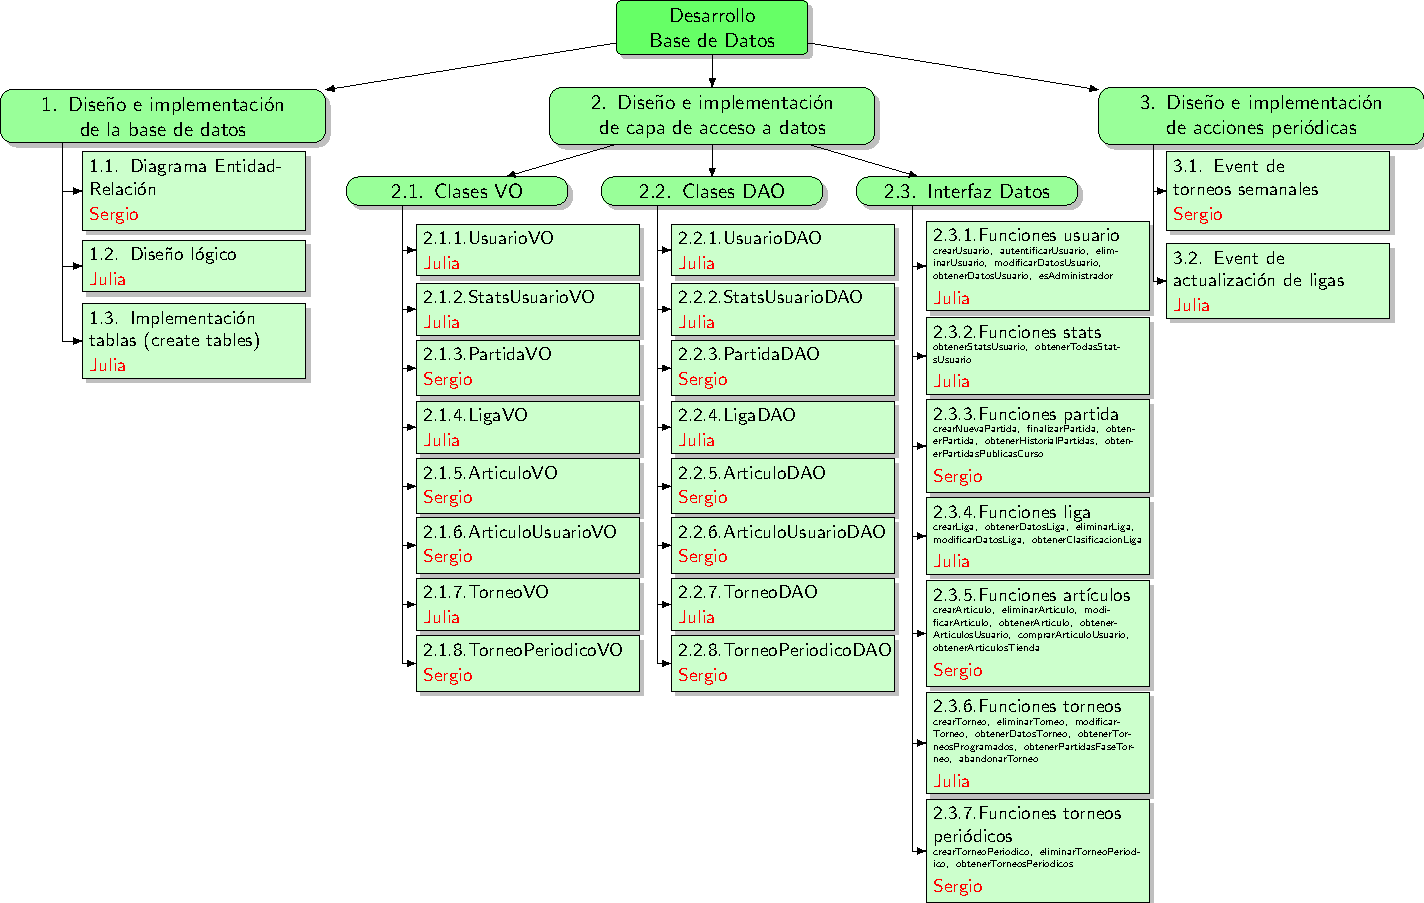
\includegraphics[scale=0.8]{figuras/edtBasesDatos.pdf}
		\caption{Diagrama de Paquetes de Trabajo Bases de Datos}
	\end{figure}

\begin{figure}[H]
		\centering
		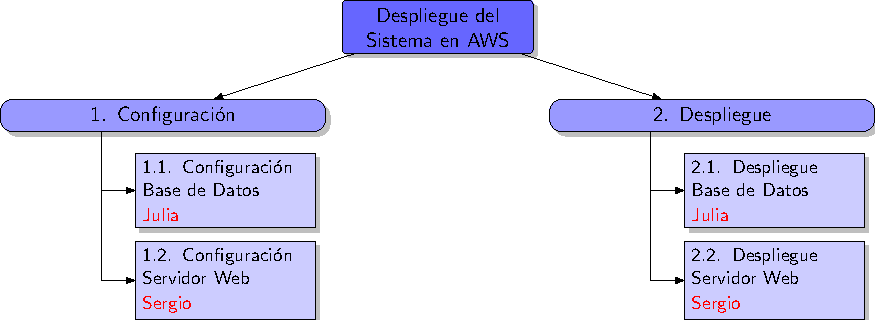
\includegraphics[scale=0.8]{figuras/edtDespliegue.pdf}
		\caption{Diagrama de Paquetes de Trabajo Despliegue}
	\end{figure}

Es importante añadir que el trabajo de integración de los diferentes paquetes de trabajo no está reflejado en estos diagramas pero también ha sido necesario repartirlo y realizarlo.
\subsubsection{Comunicación interna}
La decisión de la nueva estructura de grupos se realizó mediante una reunión entre los miembros afectados por el cambio.
En cuanto a la parte de BackEnd, al comienzo del proyecto la comunicación ha sido bastante pobre, ya que en algunos momentos los desarrolladores han realizado la misma actividad por duplicado. En el desarrollo de los diferentes componentes cada miembro tenía su propio diseño en mente y ha sido necesario ponerse de acuerdo y plasmar el diseño en un diagrama UML de clases, que todos pudieran consultar y hacer referencia. Hacia el final de la primera iteración el equipo ha mejorado su comunicación en gran medida.
\\
La comunicación entre los diferentes equipos se ha llevado a través del servicio de terceros Skype para, principalmente, resolver dudas acerca de como comunicar e integrar las distintas partes de la aplicación. Además, se utiliza el servicio de mensajería WhatsApp para reportar bugs, incidencias y comonunicaciones asíncronas. También se han llevado a cabo varias de tipo presencial reuniones para especificar interfaces comunes para facilitar la integración
\\
Se ha utilizado Floobits para la programación por parejas para las partes de la aplicación más complejas.

\subsubsection{Adecuación a las herramientas y tecnologías}
% \subsubsection*{Base de Datos}
La base de datos se ha desplegado en el gestor elegido en un primer momento, MySQL en Amazon Aurora. Para la implementación se eligió Java como lenguaje de programación lo que ha permitido la utilización de librerias para la conexión de la base de datos (JDBC y c3p0). El desarrollo en Java fue acompañado del software IntelliJ que permitía el soporte para las librerías y el control de versiones. Además permite programar en Java, por lo que el uso de la herramienta es una ventaja.
\\

% \subsubsection*{FrontEnd y Middleware}
En cuanto al desarrollo de la interfaz de juego se ha utilizado la herramienta WebStorm, que permite de forma fácil hacer cambios en la interfaz y verlos reflejados de manera inmediata en el navegador. A su vez, se ha tenido que acompañar del software IntelliJ, para poder probar el funcionamiento del juego ya que se necesita del despliegue de la aplicación en Tomcat para poder probar las comunicaciones entre jugadores.
\\
% \subsubsection*{BackEnd}
Para el diseño de los diagramas de clases se ha utilizado la herramienta StarUML, la web draw.io y excel para los diagramas de las pruebas de caja blanca y las tablas para las pruebas de caja negra.
Se ha utilizado un plugin Floobits de Intellij para la programación en parejas ya que nos permitía trabajar remotamente a dos o más miembros sobre el mismo fichero en tiempo real utilizando dos cursores diferentes. Esta herramienta se ha utilizado para los métodos más difíciles como por ejemplo lanzarCarta de la clase EstadoPartida.
El principal problema encontrado fue que la tecnología utilizada ya que Java funciona con asociación dinámica. Todos los parámetros y tipos devueltos por las funciones son punteros. Esta característica hace que la encapsulación de los objetos desaparezca. Cuando se devuelve cualquier clase como resultado de un método, es necesario crear una replica exacta del objeto en memoria, para que el usuario no modifique los atributos privados de la clase. Por ejemplo, la clase logica\_partida debe devolver una copia exacta de su atributo interno estado\_partida con cada operación. Si en lugar de realizar una copia devuelve un puntero, un usuario externo puede modificar dicho estado con las funciones públicas de la clase estado\_partida clase.
\\
Uno de los principales problemas al trabajar con IntelliJ ha sido que el equipo olvida en ocasiones que no se debe subir el archivo de configuración, ya que incapacita al resto del equipo para trabajar y se ha de eliminar de forma manual.

\subsubsection{Control de versiones}
\subsubsection*{FrontEnd y Middleware}
En cuanto al control de versiones, no ha habido ningún problema grave. Si algún miembro de un equipo modifica algún fichero de otro equipo, el commit que se realice especifica de forma clara y directa que es lo que ha modificado. Para cambios grandes se pone en contacto con el responsable del equipo para solucionar el problema.
\subsubsection*{Base de Datos}
El mayor problema encontrado consecuencia de la utilización del control de versiones fue debido a la existencia de un fichero \textit{properties} con la información privada de acceso a la base de datos, que no debía de estar subida al repositorio público. Al no existir ese fichero en un repositorio público, se tuvo que compartir de forma privada y cada usuario colocó el fichero en lugares distintos, provocando errores al compilar dependiendo de la ruta del fichero.
\subsubsection*{Integración y despliegue}
En cuanto a la integración entre el acceso a datos y el backend, se detectó un claro problema de comunicación entre los grupos a mitad del desarrollo debido a que no existía una interfaz definida de forma precisa desde un primer momento. Únicamente se había comentado una interfaz ambigua que diferentes partes entendían de forma distinta, y que además, sin las definiciones concretas de las funciones, impedía llevar a cabo el desarrollo en paralelo. Cuando se detectó el problema, hubo una reunión entre ambos grupos para definir esta interfaz de acceso a los datos. Gracias a este incidente se ha aprendido la importancia del desarrollo de interfaces entre los distintos componentes de los sistemas.
El despliegue del servidor de bases de datos se realizó en AWS sin mayores problemas. En cuanto al despliegue del servidor web hubo problemas debido a una configuración de red de la máquina virtual. Tras localizar el problema se pudo solventar y finalmente acceder al servidor mediante SSH sin problemas.

Para desplegar la aplicación web, se ha utilizado el servidor Tomcat en local junto con la herramienta IntelliJ. Surgieron problemas con las versiones de Tomcat por lo que hubo que adaptar el código para que funcionara en la última versión. En cuanto a la parte jugable, se despliega directamente con la herramienta WebStorm y se ejecuta en el navegador Chrome.

\subsubsection{Pruebas del software}
\subsubsection*{FrontEnd y Middleware}
Para probar la interfaz de juego se ha utilizado la herramienta Jasmine \footnote{ \url{https://jasmine.github.io/} }, que permite hacer tests unitarios en JavaScript. Se ha creado un protipo de una partida de prueba y se comprueba que el software pasa todos los tests diseñados.

Al tratarse de un videojuego, es difícil abordar todos las posibles situaciones de la partida, por lo que para probarlo, se hace el trabajo similar al de un tester, donde juega partidas y fuerza situaciones que se salen de lo normal para comprobar el comportamiento de la partida. Cuando se detecta algún bug, se notifica a través de un issue en GitHub para que el equipo causante del mismo lo solucione.

\subsubsection*{Bases datos}
La base de datos implementada en MySQL fue probada mediante la inserción de datos falsos de ejemplo, y la realización de consultas sencillas sobre ella, que garantizan el correcto funcionamiento. La interfaz de acceso a datos ha sido probada mediante pruebas unitarias. Se desarrolló un programa de pruebas al final del desarrollo de cada clase DAO, probando función a función sobre los datos de ejemplo introducidos, y solucionando errores de implementación. Para comprobar el funcionamiento de las clases a una escala mayor se escribió un programa en Python que generaba el código de Java que probaba la base de datos insertando nuevos datos. De esta forma también se tiene la base de datos poblada con datos de apariencia real, lo que puede ser beneficioso para pruebas de otros equipos.

\subsubsection*{Progreso y Divergencias frente a la planificación inicial}
\subsubsection*{FrontEnd y Middleware}
Para la primera iteración era necesario tener funcional el juego del guiñote. El resultado ha sido que se ha realizado una versión básica funcional jugable a través de interfaz. Sin embargo, se ha dejado para la segunda iteración el requisito de cambio de dispositivo y de personalización del juego principalmente. Además, se garantizó que el modo espectador debía estar implementado. Sin embargo, no está desarrollado plenamente. La situación actual de la implementación de dicho requisito está casi terminada, a falta de la integración con la comunicación entre capas y las pruebas correspondientes.

El matchmaking y la web dinámica debería estar empezado para la primera iteración. El resultado es que se tienen las ventanas de creación y login del usuario, por lo que faltan el resto de las ventanas del mapa de navegación por implementar. El motivo del retraso ha sido que se ha subestimado el coste en tiempo de la implementación de la comunicación y el de la interfaz del juego, ya que se desconocía la tecnología con la que se iba a implementar.

En la estimación de los costes se había especificado que la interfaz eran 30 horas, pero debido los problemas que el equipo se ha tenido que enfrentar como el desconocimiento y la integración con capas inferiores, se ha superado el coste inicial.

\subsubsection*{BackEnd}
El equipo ha cumplido el diagrama de Gantt en el apartado de implementación de lógica del juego. Si bien es cierto que se ha logrado con un retraso de media semana. Puesto que el equipo se centró en la implementación de la lógica la parte de desarrollo de la web dinámica no ha cumplido el calendario impuesto al comienzo del proyecto y arrastra un leve retraso que deberá ser compensado en la segunda iteración. El retraso se debe a la gran cantidad de trabajo asignado en la planificación inicial, muy superior a la capacidad del equipo.

\subsubsection*{Bases datos}
En general se ha cumplido el diagrama de Gantt establecido, exceptuando la implementación del acceso a datos relacionado con los torneos, que estaba planificado para la primera iteración y se debe alargar a la segunda, sin suponer ningún problema de dependencias con el resto de componentes del sistema. También se puede comentar que, en lo que respecta al diseño de la base de datos, se requirió algo menos tiempo del estimado (se finalizó con una semana de antelación), mientras que el diseño del acceso a datos requirió más tiempo del estimado por lo que fueron compensados, cumpliendo bastante bien la planificación inicial.



\section*{Anexo I. Glosario}
\begin{description}
\item[Amazon AWS:] Amazon Web Services, plataforma cloud ofrecida por Amazon. \cite{aws}
\item[Amazon RDS Aurora:] Servicio de creación y mantenimiento de bases de datos relacionales. \cite{aurora}
\item[Amazon EC2:] Servicio de servidores privados virtuales de AWS que permite lanzar máquinas virtuales con los sistemas operativos y configuraciones deseadas. Además, permite contratar más o menos recursos bajo demanda, adaptándose así a los picos de carga. \cite{ec2}
\item[PostgreSQL:] es un sistema de gestión de bases de datos relacional orientado a objetos y libre, publicado bajo la licencia PostgreSQL.
\item[MySQL:] es un sistema de gestión de bases de datos relacional desarrollado bajo licencia dual: Licencia pública general/Licencia comercial por Oracle Corporation.
\item[Guiñote:] Juego de cartas español en el que pueden participar dos jugadores o dos parejas de jugadores. Se utiliza la baraja española de 40 cartas con cuatro palos. A continuación se explican detalladamente las reglas del juego:
\begin{itemize}
\item{El juego comienza repartiendo 6 cartas a cada jugador y colocando una carta en medio del tapete que determina el palo que es "triunfo". La manera de jugar es por rondas denominadas bazas, en las que cada jugador tira una carta. La baza se gana si se tira el triunfo más alto, o si no hay triunfo, si se tira la carta con mayor valor del palo de la carta de salida. Al ganar la baza, se suma a la puntuación de la pareja o el jugador el valor de las cartas. Además si se gana la baza se puede intercambiar el siete del palo de triunfo por la carta que se encuentra en medio del tapa si su valor es superior a la del siete, o también se puede sumar puntuación si el jugador tiene un "cante" que significa que el jugador posee la sota y el rey de un mismo palo, lo cual da 20 puntos si el palo no es triunfo y 40 puntos si el palo es triunfo.}
\item{El valor de las cartas de forma decreciente es el siguiente: As (11 pts), tres (10 pts), rey (4 pts), sota (3 pts), caballo (2 pts), siete (0 pts), seis (0 pts), cinco (0 pts), cuatro (0 pts) y dos (0 pts).}
\item{Después de cada baza, y mientras queden cartas en el mazo, cada jugador roba una carta empezando por el jugador que se haya llevado la última baza. Tras esto, será el primer jugador en jugar la primera carta de la siguiente baza.}
\item{Una vez que se acaban las cartas para robar se introducen restricciones a la hora de tirar las cartas. El primer jugador en tirar no tiene restricciones pero el resto de jugadores deberá tirar una carta del mismo palo o si no tiene, triunfo, además de que está obligado a "matar", es decir, tirar una carta para intentar ganar la baza. En caso de que el jugador no pueda cumplir ninguna de estas restricciones con las cartas que posee puede tirar la carta que desee. Finalmente, el equipo que gane la última baza ganará 10 puntos extra.}
\item{Para determinar quién ha ganado, se suma la puntuación y gana el jugador o la pareja que supere los 100 puntos (divididos habitualmente en 50 “malas”, los primeros 50 puntos, y 50 “buenas”, los restantes). En caso de que nadie supere la anterior cifra se vuelve a repartir y a cada baza que se gana se incrementa la puntuación hasta que se llega a 100, momento en el que se gana. En el caso de que ambos equipos superasen los 100 puntos en la misma jugada, ganaría aquel que hubiese ganado la última baza.}
\end{itemize}
\end{description}
\addcontentsline{toc}{section}{\protect\numberline{}Anexo I. Glosario}%
\newpage
\bibliographystyle{abbrv} % We choose the "plain" reference style
\bibliography{data}
\end{document}
